\documentclass[11pt,a4paper,english]{book}  % book, article

\usepackage[english]{babel}
\usepackage[utf8]{inputenc}
% Paquetes para incluir graficos:
\usepackage{graphics}
\usepackage{graphicx}
\usepackage{epstopdf}
% Tratamiento de graficos
\usepackage{picture}
% Colores
\usepackage[usenames]{color}
% Texto preformateado
\usepackage{verbatim}
\usepackage{listings}
% Hipervinculos (indice y URLs)
\usepackage{hyperref}
% Matematicas
\usepackage{amsfonts}
\usepackage{amsmath}
\usepackage{mathtools}
\usepackage{amsthm}
\usepackage{amssymb}
\usepackage{anysize}
\usepackage{caption}
\usepackage{geometry}
\usepackage[final]{pdfpages}
\usepackage{cite}
\usepackage{natbib}
\usepackage[numbib,notlof,notlot,nottoc]{tocbibind}
\usepackage{mathtools,xparse}

\newcommand{\HRule}{\rule{\linewidth}{0.5mm}}

%%PER EL CODI EN C%%%
\usepackage{listings}
\lstset{ %
language=C++,                % choose the language of the code
basicstyle=\footnotesize,       % the size of the fonts that are used for the code
numbers=left,                   % where to put the line-numbers
numberstyle=\footnotesize,      % the size of the fonts that are used for the line-numbers
stepnumber=1,                   % the step between two line-numbers. If it is 1 each line will be numbered
numbersep=5pt,                  % how far the line-numbers are from the code
backgroundcolor=\color{white},  % choose the background color. You must add \usepackage{color}
showspaces=false,               % show spaces adding particular underscores
showstringspaces=false,         % underline spaces within strings
showtabs=false,                 % show tabs within strings adding particular underscores
frame=single,           % adds a frame around the code
tabsize=2,          % sets default tabsize to 2 spaces
captionpos=b,           % sets the caption-position to bottom
breaklines=true,        % sets automatic line breaking
breakatwhitespace=false,    % sets if automatic breaks should only happen at whitespace
escapeinside={\%*}{*)}          % if you want to add a comment within your code
}

%%%%%%%% Entornos teorema, definiciÛn, comentario, ... %%%%%%%%
\swapnumbers  % Poner el numero del teorema ANTES del teorema.

\theoremstyle{definition}  % Titulo en negrita y texto plano

\newtheorem{definicion}{Definicion}[chapter]
\newtheorem{ejemplo}[definicion]{Ejemplo}
\newtheorem{comentario}[definicion]{Comentario}
\newtheorem{propiedades}[definicion]{Propiedades}
\newtheorem*{objetivo}{Objetivo}
\newtheorem*{idea}{Idea}

\theoremstyle{plain}  % Titulo en negrita y texto en cursiva.
\newtheorem{teorema}[definicion]{Teorema}
\newtheorem{proposicion}[definicion]{ProposiciÛn}
\newtheorem{corolario}[definicion]{Corolario}
\newtheorem{lema}[definicion]{Lema}

\theoremstyle{remark}  % Titulo en cursiva y texto plano
\newtheorem*{observacion}{ObservaciÛn}
\newtheorem*{ejercicio}{Ejercicio propuesto}
\newtheorem*{pregunta}{Pregunta}

%%%%%%%% Formato cÛdigo incluido %%%%%%%% 
\lstset{ %
%language=Octave,                % choose the language of the code
basicstyle=\footnotesize,       % the size of the fonts that are used for the code
numbers=left,                   % where to put the line-numbers
numberstyle=\footnotesize,      % the size of the fonts that are used for the line-numbers
stepnumber=1,                   % the step between two line-numbers. If it's 1 each line 
                                % will be numbered
numbersep=5pt,                  % how far the line-numbers are from the code
%backgroundcolor=\color[rgb]{0.8,0.8,0.8},  % choose the background color. You must add \usepackage{color}
showspaces=false,               % show spaces adding particular underscores
showstringspaces=false,         % underline spaces within strings
showtabs=false,                 % show tabs within strings adding particular underscores
frame=single,	                % adds a frame around the code
tabsize=2,	                % sets default tabsize to 2 spaces
captionpos=b,                   % sets the caption-position to bottom
breaklines=true,                % sets automatic line breaking
breakatwhitespace=false,        % sets if automatic breaks should only happen at whitespace
title=\lstname,                 % show the filename of files included with \lstinputlisting;
                                % also try caption instead of title
escapeinside={\%*}{*)},         % if you want to add a comment within your code
morekeywords={*,...}            % if you want to add more keywords to the set
}





\newgeometry{
    top=35mm,
    bottom=30mm,
    outer=30mm,
    inner=30mm,
}

\begin{document}


\begin{titlepage}
\begin{center}


\textsc{\LARGE Kungliga Tekniska Högskolan}\\[1.5cm]

\textsc{\Large ~}\\[-0.5cm]


{ \huge \bfseries \textbf{Project Report} \\

\HRule

 Noise cancellation in a teleconference\\[0.4cm]}

\HRule \\[1.1cm]

		\begin{figure}[h]
		\centering
		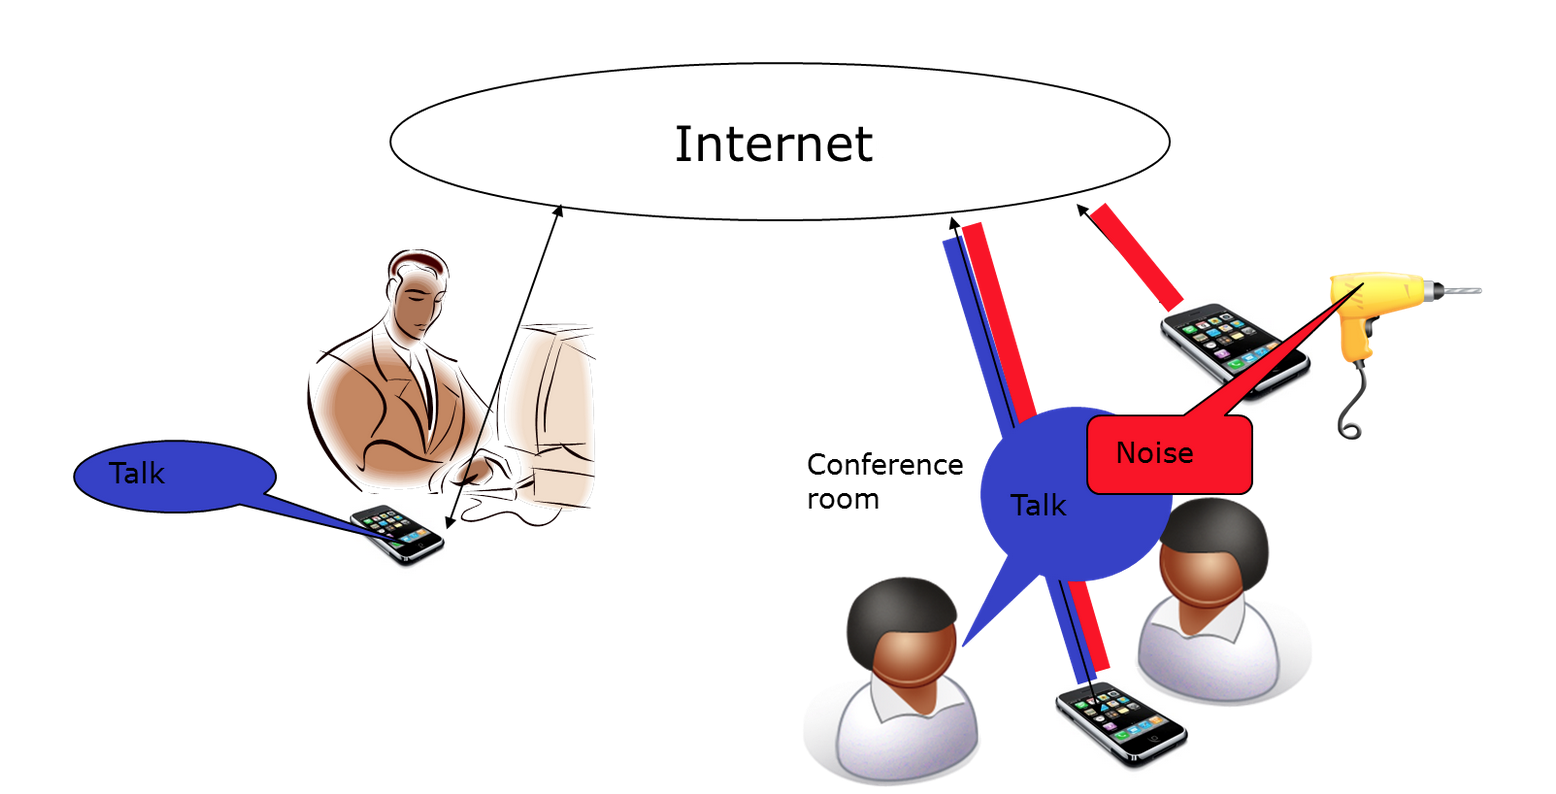
\includegraphics[width=10cm]{images/other/scenario}
		\label{scenario}
		\end{figure}

% Author and supervisor
\begin{minipage}{0.4\textwidth}
\begin{flushleft}
\emph{Authors:}\\
Animesh DAS \\ Jonas SEDIN \\ Mohammad ABDULLA \\ Thomas GAUDY \\ Xavier BUSH
\end{flushleft}
\end{minipage}
~
\begin{minipage}{0.4\textwidth}
\begin{flushright}
\emph{Advisor:}\\
Per ZETTERBERG
\end{flushright}
\end{minipage}

\vfill

% Bottom of the page
{\large Spring 2015} \\[1cm]
\end{center}



\end{titlepage}
\restoregeometry


\pagebreak\tableofcontents
\pagebreak

\chapter{Background}

	\section{Introduction of noisy environments}
	\label{sec:intronoise}
	
It is a fact that the scenarios with phone calls involved are increasing every day. This situation implies an increase of the probability of being in a noisy scenario, specially in big cities. As a result of the discomfort that the users suffer in these noisy environments, engineering and science have worked with different approaches to solve this problem.

The diversity of noise nature and its sources lead the engineering to a big challenge: develop high performance soltions in these diverse environments. When facing noise cancellation is very important to take into account the variability that the noise may experience, as previously said. Duration of the noise sequences (from \textit{ms} to long sequences), color of the noise and stationarity are possible classifications of the noise and each classification implies different ways of treating it. Therefore, a lot of systems are using combined techniques to reach the best possible performance, which has been naturally the case of this project.

	\section{Historical Overview}
	\label{sec:historia}
	Before presenting the proposed solutions and approaches of the project, it is needed a historical overview to understand how have the group been influenced and which have been the patterns of research.
	
	The first recognized work on eliminating noise from speech signal was documented in 1934 when Paul Lueg was granted the first patent for a noise control system. In his work, Paul Lueg explained his way to cancel sinusoidal tones in ducts by phase-advancing the wave and then by inverting the polarity to cancel random sounds in the area nearby an amplifier. Basically he developed a process of silencing disturbing sound oscillations or noise which was able to work independently of the main source of oscillation or speech \cite{patent1}. 
	
After this work of Paul Lueg, a lot of people started working on improving noise cancelation technique used by Paul and later in 1950, Lawrence J. Fogel designed a systems where he successfully canceled the noise in helicopter and airplane cockpits communication. This work of Lawrence J. Fogel was a milestone in the noise cancellation system development where he designed a system for supplementing a standard noise suppressor by eliminating the peaks of energy as well as the nulls of energy. He claimed his design to be able to increase the lucidity of speech in noisy environment significantly over the works done previously \cite{patent2}.

Meanwhile Willard Meeker was working to implement active noise control to a circumaural earmuff and in 1957 he successfully developed a working model of his headset with an active attenuation bandwidth of approximately \textit{50–500 Hz} and a maximum attenuation of approximately 20 dB \cite{online3}.
During 1980’s due to the technological boom, travelling less and doing the meetings over telephone became an efficient way to reduce the pressure on our environment and do business more economically. At that time technology present to reduce the noise from the speech signal was not efficient enough to make a perfect teleconference without any noise interference issue. As a consequence, more private researchers and companies were interested to develop more advanced working design to cancel noise efficiently to have a completely noise-free environment for teleconference or other communication systems. 

In 1980, one highly recognized work on this field was that of S. Boll of University of Utah, who was successful to efficiently suppress the acoustic noise in speech using two microphone adaptive noise cancellation system. He used least mean square (LMS) and the lattice gradient algorithms to suppressed acoustic noise with energy greater or equal to the speech by adaptively filtering a separately recorded correlated version of the noise signal and then subtracting it from the speech waveform. Both methods were able to decrease ambient noise power by at least 20 dB with insignificant speech distortion and therefore was powerful enough to work as noise suppression preprocessors for voice communication in severe noise environments \cite{supression}.

Another work of 1980’s which is still one of the best techniques used for speech enhancement is the work of Y. Ephraim and D. Malah, which was published April 1985. They have developed a highly efficient Short-Time Spectral Amplitude (STSA) estimator for speech signals to minimize the mean square error of the log-spectra. Actually this work was an enhancement of their previous work titled “Speech Enhancement Using a- Minimum Mean-Square Error Short-Time Spectral Amplitude Estimator” published in December 1984. They formulated the STSA by estimating the amplitude of each Fourier expansion coefficient of the speech signal, given the noisy process in the interval [0, T]. Their Gaussian statistical model was motivated by the central limit theorem, as each Fourier expansion coefficient is basically a weighted sum (or integral) of random variables resulting from the process samples. Eventually they were able to have lower residual noise level without hampering the speech itself taking the signal presence uncertainty into account \cite{speech} \cite{logmmse}.

Since then there has been lot of work going on reducing noise in speech signal. Later on 1992, G. Mirchandani, R. Zinser Jr. and J.B. Evans developed a structure for joint process estimation for noise canceling, when the reference signal is contaminated with crosstalk. They have done the simulation as per their design with the transversal and the lattice-based CTRANCs, and they have found out that for 1 to 9 dB levels of crosstalk, their design shows 3 to 11 dB improvement in the mean-square error over that for the standard adaptive noise canceller \cite{crosstalk}.

After going through several works of various scholar of different time and research field including the works mentioned above as well, we have decided to study more on this topic and develop a design to appropriately apply noise cancellation in such a way which enables the system to extract only the voice signal removing as much noise as possible. After discussing with our project supervisor Prof. Per Zetterberg we have decided to go ahead with this project with our previous knowledge gained from the Adaptive Signal Processing course. In the adaptive signal processing course, different adaptive signal processing algorithms were unmasked to us for extracting relevant information from noisy signals where the emphasis was mainly on recursive, model based estimation methods for time-varying systems. 

Finally, \textit{Adaptive Signal Processing} came up with the first theoretical proposals in the 1960's. This field of signal processing embraces several algortihms such Lest Mean Squares (LMS), Recursive Lest Squares (RLS) and Kalman Filtering. These are the algorithm that will take place with more relevance further in this report.



	\section{Description of the project}
	\label{sec:introproblem}
	
	The problem proposed by the course \textit{EQ2440} has been a "Noise and echo cancellation of a teleconference". The general scenario is that the first of the two speakers of the teleconference is in a noisy environment and the clear goal is to cancel as much noise as possible in order that the second speaker could receive a cleaner speech and make the conversation more comfortable. As said in \ref{sec_intronoise}, there are different approaches to solve this problem, where several of them require the availability of pure noise recordings, in our case recorded with a third phone placed close to the noise source. To have a clearer overview of the scenario the Figure \ref{scenario2} shows an approximate scheme easy to understand.
	
	When talking about denoising a teleconference there are two factors to take into account, techniques to cancel the noise and the possibility of their implementation in a real time application. The real time application has been, as expected, a big challenge because it implies good performance in terms of cancellation with the minimum reachable delay to conserve the naturalness of the conversation.
	
		\begin{figure}[h]
		\centering
		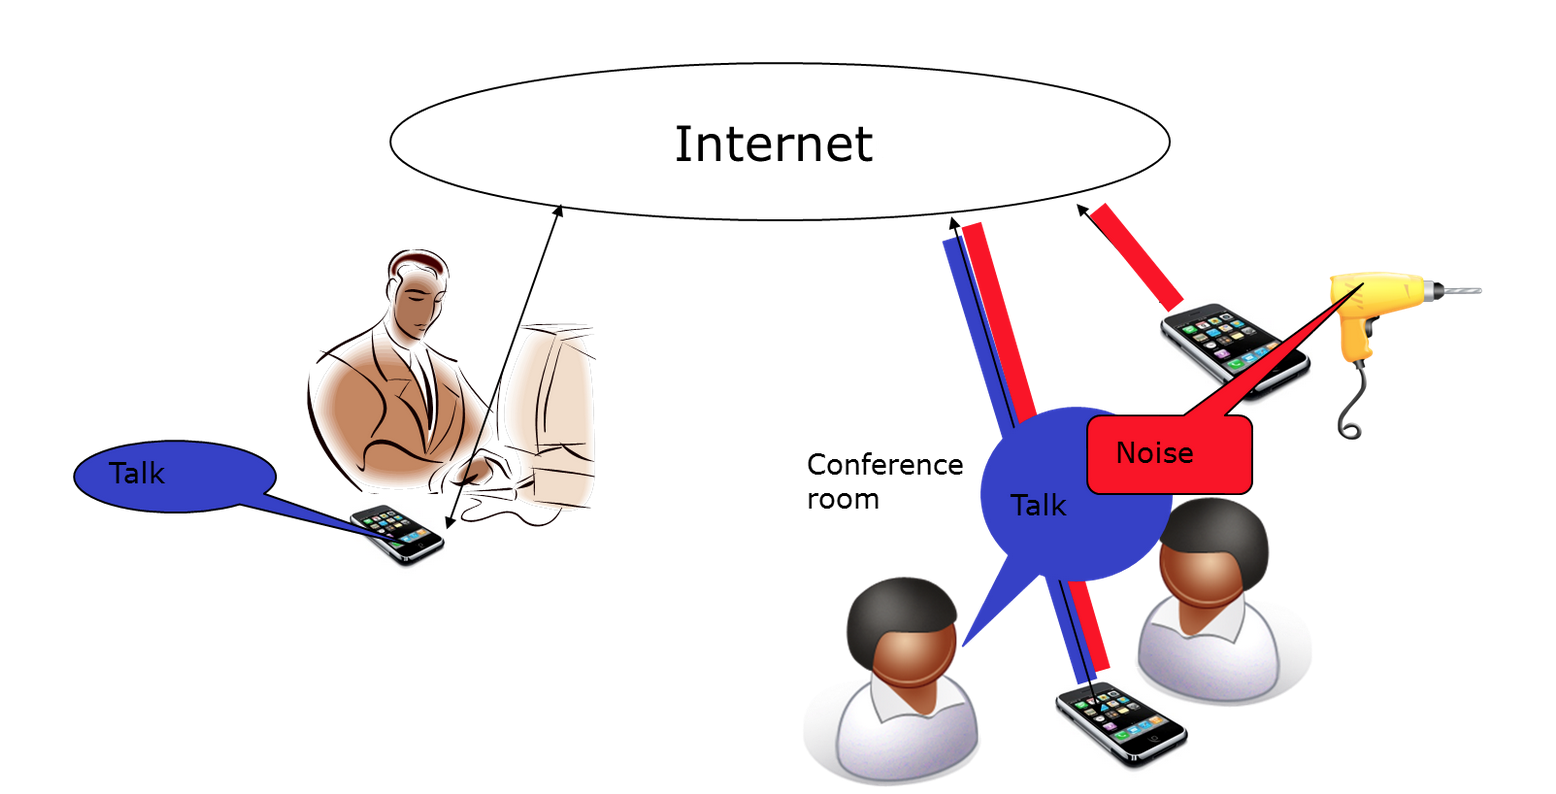
\includegraphics[width=10cm]{images/other/scenario}
		\caption{Scenario to solve}
		\label{scenario2}
		\end{figure}
	
	
	
	\section{Goal}
	As commented in \ref{sec:introproblem}, the goal is to cancel the noise contribution in the conversation between the two speakers of the teleconferences. With the purpose to simplify the scenario, it will be assumed that only one of the speakers is surrounded by noise and the main noise source is known as well.
	
	As in every engineering project, the group had to find a compromise between performance in noise cancellation and viability of implementation in real life. As it will be explained in \ref{sec:methodology}, the computational cost is a big constrain and the best performance of certain approaches (\ref{sec:theory}) introduce too much delay because of this reason. As a consequence, not always the best solution will be possible to implement in the real time version of the project.
	
	As a contrast, the personal goals of the project members are to learn form the teamwork environment, learn a research methodology, research criteria and certain skills of management that might be used in the performance of a Master Thesis (as an inmidate future) and in a research or business environment.
	
	The new knowledge acquisition is obviously another personal goal of all the team members.
	
	
	\section{Organizationn and Human Resources}
	\label{organization}

The organization of the project consists in electrical engineering students at different stages of the studies and within different specializations. In order to make the team as efficient as possible, the project has been divided in four different groups: \textit{Theory Group}, \textit{Android Group}, \textit{Multimedia Group} and \textit{Management Group}, all of them explained in detail in \ref{sec:methodology}.

The distribution of the team members has been as follows.

\begin{itemize}

\item Animesh Das
	\begin{itemize}
	\item Role: Management Group
	\item e-mail:animeshu1989@gmail.com (animeshd@kth.se)
	\item Telephone: +46 737155575
	\end{itemize}
	
\item Jonas Sedin
	\begin{itemize}
	\item Role: Theory Group \& Android Group
	\item e-mail: sedinjo@gmail.com (jonassed@kth.se)
	\item Telephone: +46 704252951
	\end{itemize}
	
\item Mohammad Abdulla
	\begin{itemize}
	\item Role: Android Group \& Multimedia Group
	\item e-mail: hamodiilatch@gmail.com (mabdulla@kth.se)
	\item Telephone: +46 737393276
	\end{itemize}
	
\item Thomas Gaudy
	\begin{itemize}
	\item Role: Android Group
	\item e-mail: gaudy.thomas@gmail.com (gaudy@kth.se)
	\item Telephone: +46 760936034
	\end{itemize}
	
\item Xavier Bush
	\begin{itemize}
	\item Role: Theory Group \& Management Group (Project Leader)
	\item e-mail: xavier.bush@gmail.com (xbush@kth.se)
	\item Telephone: +46 764141834
	\end{itemize}
	
	
\end{itemize}

The sponsor members as Project Examiner/Supervisor and Project Support are:

\begin{itemize}
\item Per Zetterberg
	\begin{itemize}
	\item Role: Project Examiner
	\item e-mail: perz@ee.kth.se
	\item Telephone: +46 8 790 77 85
	\end{itemize}
	
\item Hadi Ghauch
	\begin{itemize}
	\item Role: Group Assistant
	\item e-mail: ghauch@kth.se
	\end{itemize}
	
\item Martin Ohlsson
	\begin{itemize}
	\item Role: Android Guru
	\item e-mail: martinoh@kth.se
	\item Telephone: +46 87907818
	\end{itemize}
\end{itemize}

\chapter{Methodology}
\label{sec:methodology}

This chapter shows the methodology that the group has followed since the projecte started. On the first hand, it goes without saying that the project group has followed the \textit{Scientific Method} in the implementation of the project. On the second hand, as commented in \ref{organization}, the group has been divided in three groups explained in the following subsections.

	\section{Theory Group}

The\textit{Theory Group} had as its main goal finding solutions to cancel the present noise in the teleconference. Nevertheless, a constraint of the group has been the computational cost that the implementation have, where all the details may be found in \ref{sec:theory}.

The fact that three members of the project had recent and good background in Adaptive Signal Processing, which has been one of the chosen approaches to face the noise cancellation, made easier the making of the groups. Moreover, the \textit{Theory Group} avoided the first stage in theory research, which is the most difficult part when starting a new project.

In terms of methodology, the \textit{Theory Group} has followed next steps:

\begin{itemize}
\item Make research in suitable algorithms.
\item Record with the given mobile phones both signals: 'voice+noise' and 'noise'. 
\item Test the performance in MATLAB.
\item Check the computational cost in MATLAB.
\item Check the possibility to transfer the solutions from MATLAB to Android.
\end{itemize}

Because of the presence of Jonas Sedin in the \textit{Theory Group} and the \textit{Android Group}, it has been possible to design theory solutions think in the availability to transfer them to Android coding.\\



	\section{Android Group}
	
	This group has had two different duties:
	
	\begin{itemize}
	\item Android tasks: these tasks aimed to be an introdution to the Android programming.
	\item Noise cancellation in Android: has been the transfer from the proposed solution in the \textit{Theory Group} to Android.
	\item Real time application: optimize the code to decrease the computational cost and make possible a real time application.
	\end{itemize}
	
	In this case, even if Thomas Gaudy has not been a part of the \textit{Theory Group}, his background in Adaptive Signal Processing has helped in the implementation of the proposed solutions.
	
	\section{Multimedia Group}

This group is only formed by Mohammad Abdulla who has taken care of all the technical preparation of the presentations of the project:

\begin{itemize}
\item Video of the project: explanation of the project with real examples.
\item Power Point Presentation: power point to use in the Grand Final Presentation.
\item Bloopers Video: video containing bloopers and funny moments during the performance of the project.
\end{itemize}

	\section{Management Group}

The \textit{Management Group} has taken care of the drawing up of those tasks that were oriented to plan, follow up and present the work of the project.

The main documents are listed below:

\begin{itemize}
\item Project Plan: document that contained a brief description of the project, time resources and planning and tasks planning.
\item Progress Report: document containing the follow up of the projects in terms of achievements and resources. It is a updated version of the Project Plan.
\item Project Report: this precise document. It contains the description of all the project in all the areas.
\end{itemize}

Besides the main documents, the \textit{Management Group} has taken care of next tasks:

\begin{itemize}
\item Meetings: there has been no need to schedule meetings because of the small size of the group and the cross-group duties.
\item  Scheduling: the planning of all the tasks was designed by this group and it has been properly followed.
\end{itemize}

As every document listed before is already available for the supervisor, in this document it is only going to be shown the last version of the Gantt Chart in Figures \ref{fig:gantt1} and \ref{fig:gantt2}.


		\begin{figure}[h]
		\centering
		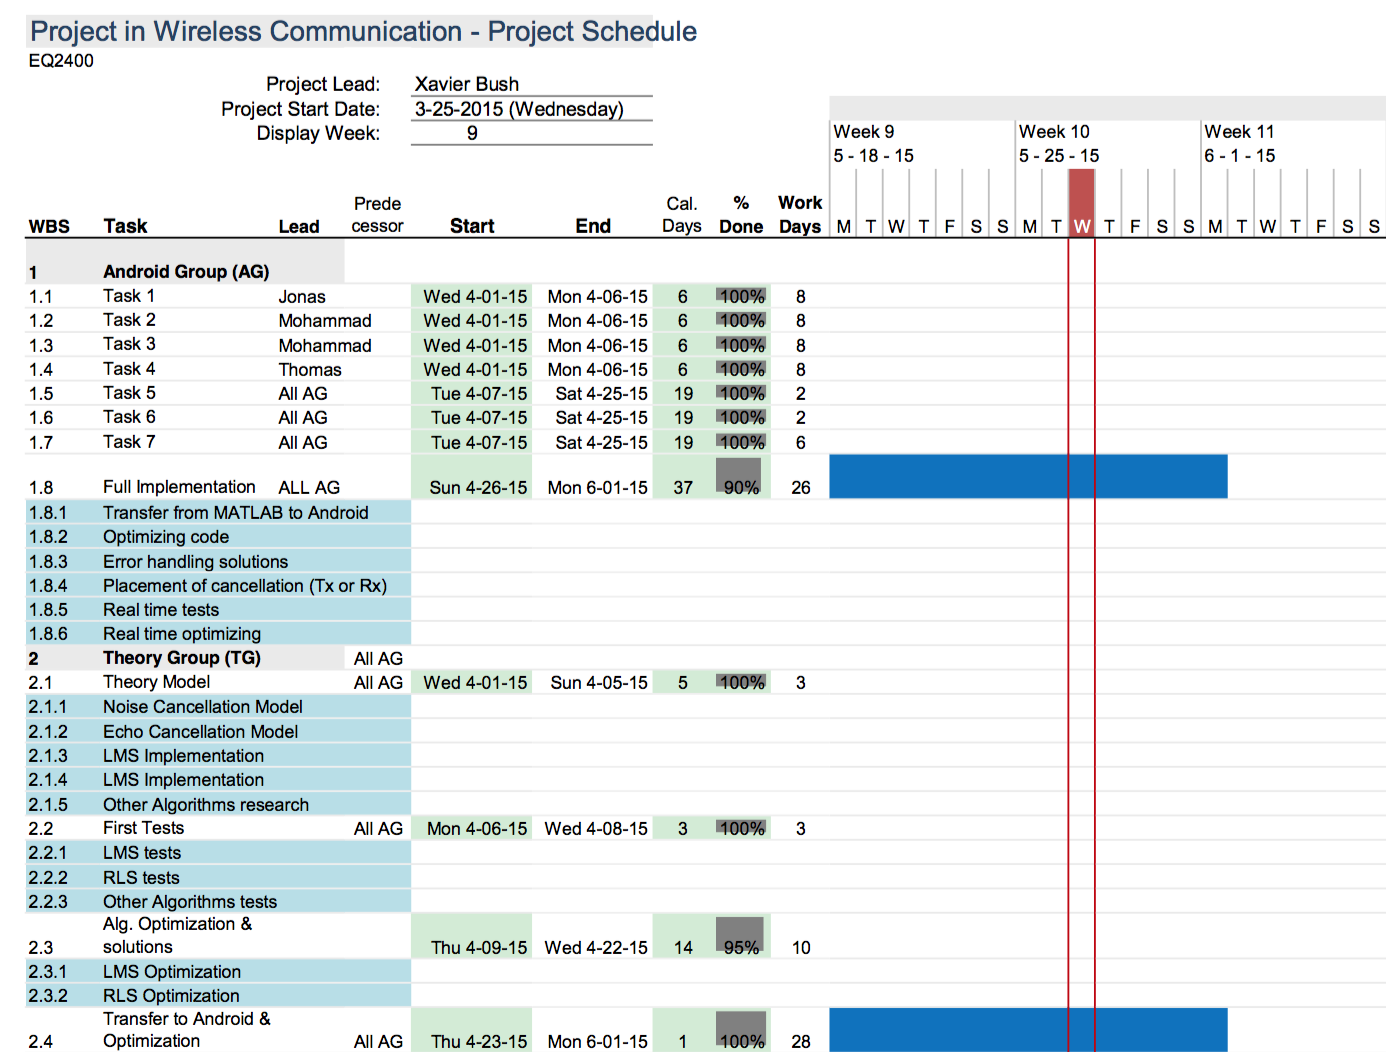
\includegraphics[width=15cm]{images/management/ganttchart1.jpg}
		\caption{Gantt Chart example}
		\label{fig:gantt1}
		\end{figure}

		\begin{figure}[h]
		\centering
		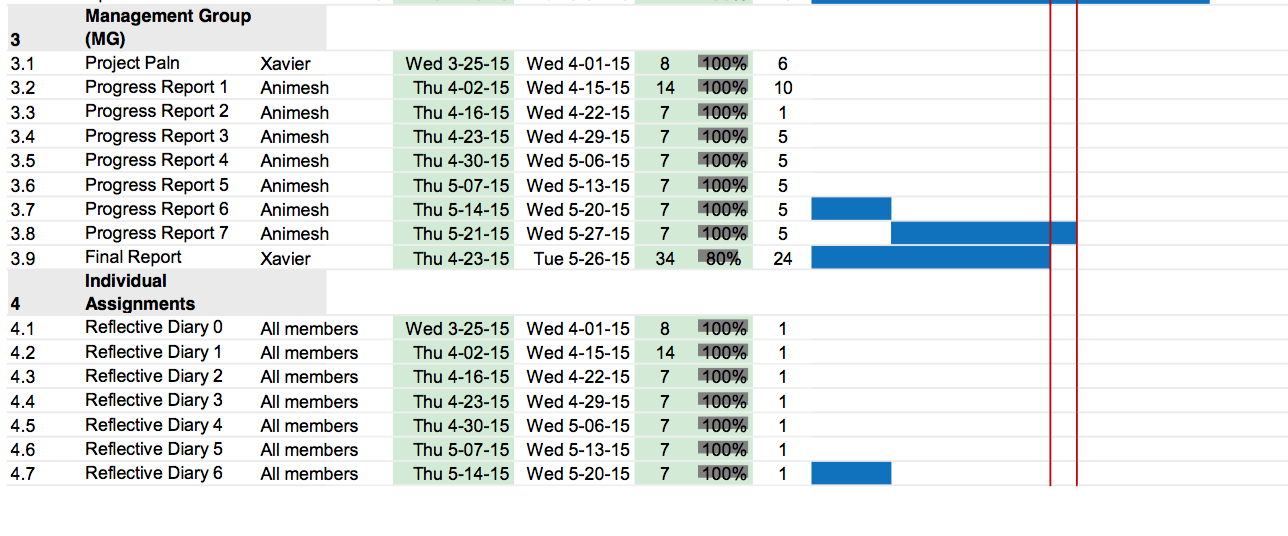
\includegraphics[width=15cm]{images/management/ganttchart2.jpg}
		\caption{Gantt Chart example}
		\label{fig:gantt2}
		\end{figure}


\section{Cross-Groups Duties}

In terms of making the transfer of information between groups easier, the makeup of the groups has followed a cross-specialization criteria. Therefore, there are team members in more than one group, and it has been possible due to the wide scope of skills that the team members have (\ref{organization}).

\chapter{Theory}
\label{sec:theory}

The \textit{Theory Group} has been working within different scenarios but mainly has followed what is called \textit{Adaptive Signal Processing}, as it has been explained in \ref{sec:history}. Some of them have ended in good performance algorithms where only two of them have been transferred to Android and some other have not reached the wanted outcome.

In terms of goals, it has been very important for the group to reach a good noise cancellation and preserving as much as possible of the voice quality.

\section{Successful Approaches}

	\subsection{LMS Algorithm}
	\label{lms}
	
		\subsubsection{Introduction}
	
	The LMS (Least Mean Square) Algorithm \cite{asp} is an adaptive filtering technique used to estimate the unwanted component in the signal that wants to be filtered and, a posteriori, subtract it to "clean" the wanted signal.
	
	To use this technique it is needed to have both signals, the one that contains the useful information ($y(n)$) and the noisy one ($x(n)$).
	
	The process used in this technique is a recursive calculation samples by sample were $N$ previous samples of the wanted signal are used to calculate the current filter sample, used later on for the subtraction.
	
	The original problem to solve in LMS is shown in the Equation \ref{eq:lmsgeneral1}, where it is clearly visible that the LMS minimizes the MSE using the instantaneous error.
	
		\begin{equation}
	\label{eq:lmsgeneral1}
		\hat{\theta}(n) = \hat{\theta}(n-1) -\frac{\mu}{2})\frac{\partial}{\partial \theta}MSE(n,\theta)\rvert_{\theta=\hat{\theta(n-1)}}
	\end{equation}
	
	Where after the appropriate calculations, the final version ready to implement in MATLAB is next:
	
	\begin{equation}
	\label{eq:lmsgeneral2}
		\hat{\theta}(n) = \hat{\theta}(n-1) + \mu Y(n)(x(n)-Y^{T}(n)\hat{\theta}(n-1))
	\end{equation}
	
	In the Equation \ref{eq:lmsgeneral2}:
	
	\begin{itemize}
	\item $\hat{\theta}(n)$: estimation of the current sample of the filter
	\item $\hat{\theta}(n-1)$: estimation of the previous sample of the filter
	\item $Y(n)$: vector that contains the $N$ samples used in the implementation
	\item $x(n$): sample of the wanted signal
	\item $\mu$: step size
	\end{itemize}
	
	A very important parameter to consider is the \textit{Step Size} $\mu$. The value of $\mu$ has a direct impact on the stability and convergence of the algorithm. The general rule of choosing the right \textit{step size} is shown in \ref{eq:stepsize}
	
	\begin{equation}
	\label{lmsmu}
	0 < \mu <\frac{2}{\lambda_{1}} 
	\end{equation}
	
	where $\lambda_{1}$ is the maximum eigen value of $I-\mu \Sigma_{YY}$.
	
	In terms of cost operations, LMS is very efficient thus only needs O(N) operations in each iteration. A priori, this is feasible for a real time implementation and this one of the reason that made us start with this approach.
	
	Nevertheless, the implementation of LMS for noise cancellation is a little bit different. As showed in Figure \ref{fig:simplms}, the purpose is to estimate $x_{1}(n)$ from $x(n)$, i.e. calculate $\hat{x_{1}}(n)$ to then subtract if from $z(n)=s(n)+x(n)$ from the received signal at the receiver phone. In conclusion, it is necessary that de \textit{Adaptive Filter} emulate the \textit{Channel}.
	
		\begin{figure}[h]
		\centering
		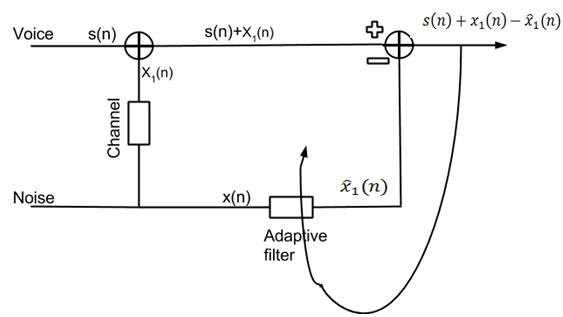
\includegraphics[width=8cm]{images/theory/SimplifiedLMS.jpg}
		\caption{Simplified boxes scheme of LMS (Noise Cancellation)}
		\label{fig:simplms}
		\end{figure}
		
		Finally, it is important to comment that for a good performance of the \textit{LMS Algorithm} it is needed a high correlation between the noise coming from the first speaker and the one coming from the phone that records the noise. To do so, a synchronisation will have to be applied in the receiver.
		
	
	\subsubsection{Implementation \& Results}
	
	The implementation used in MATLAB is based on the one that Jonas, Thomas and Xavier have done during the course of \textit{Adaptive Signal Processing (EQ2400)}.
	
	Once all the recordings where done, the first tests of the LMS gave different performances depending on the number of previous samples used to calculate the filter.
	
	\begin{itemize}
	\item $N=100$: good performance
	\item $N=1000$: better performance with a big computational cost
	\end{itemize}
	
	Even though there is an upper limit for the value of $\mu$ (\ref{eq:lmsus}), there is not a lower limit (besides $0$). Therefore, the group followed a test-and-set empirical criteria where different $\mu$ values where tested and the value who gave the best auditive performance was the chosen. In the last case, the best performance was given by $\mu=5 \cdot 10^{-5}.$
	
	These results are reasonable: if seems that the bigger filter is used the more noise cancellation is achieved. However, there is a reverberation introduced when using big filters.
	
	To show some graphic results of the performance of this algorithm, on the one hand Figure \ref{fig:lmstime100} and \ref{fig:lmsfreq100} show the time and frequency response of the filtered sequence with $N=100$ samples in comparison with the original recording. There is some audible noise reduction that in the figure can be seen in the noisy frames where there is more presence of noise in the original plot than in the filtered one. When it comes to the frequency domain, we can appreciate that there are several small peaks at low frequencies and the contribution of the peak at $f=0.6$ (where $fs=44.1$ KHz) has been slightly decreased.
	
	On the other hand,  the Figures \ref{fig:lmstime1000} and \ref{fig:lmsfreq1000} show the same comparison as before but with a filter of $N=1000$ samples. In this case the Figure \ref{fig:lmstime1000} shows that the noise has less presence. The drawback comes with a certain distortion in the audio file that can be seen in the Figure \ref{fig:lmsfreq1000} as a modification in the frequency domain with new peaks in a coarser spectral response at lower frequencies.
	
	In terms of computational time, in MATLAB the LMS with $N=100$ samples takes 2.22 seconds, while the LMS with $N=1000$ takes 3.78 seconds (increasing of a 70\%). This does not make a huge difference in MATLAB but in a real time application it might, therefore it will be treated by the \textit{Android Group}.
	

	As a clarification, the reason why the group has tested different number of samples in the LMS is because the lack of synchronization between $z(n)$ and $x(n)$: with a bigger N the delay between both signals is solved in terms of filtering.
	
		\begin{figure}[h]
		\centering
		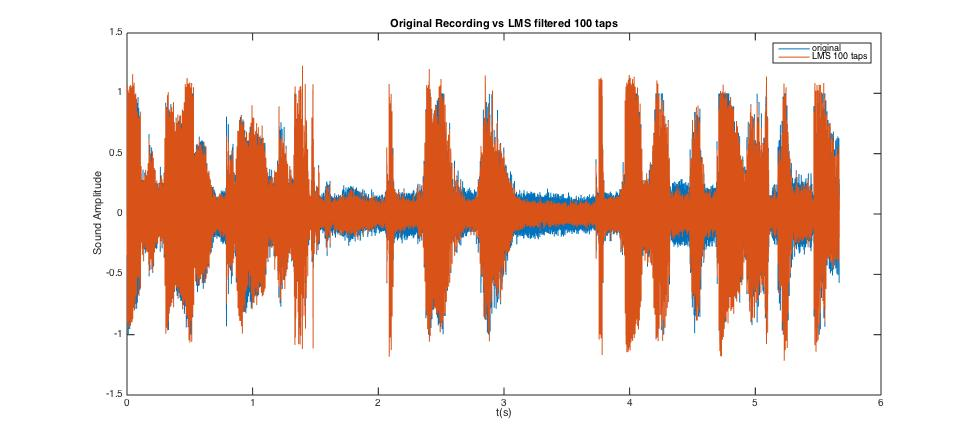
\includegraphics[width=15cm]{images/theory/lms100tapstime.jpg}
		\caption{Time Domain - LMS result with N=100}
		\label{fig:lmstime100}
		\end{figure}
		
		
		\begin{figure}[h]
		\centering
		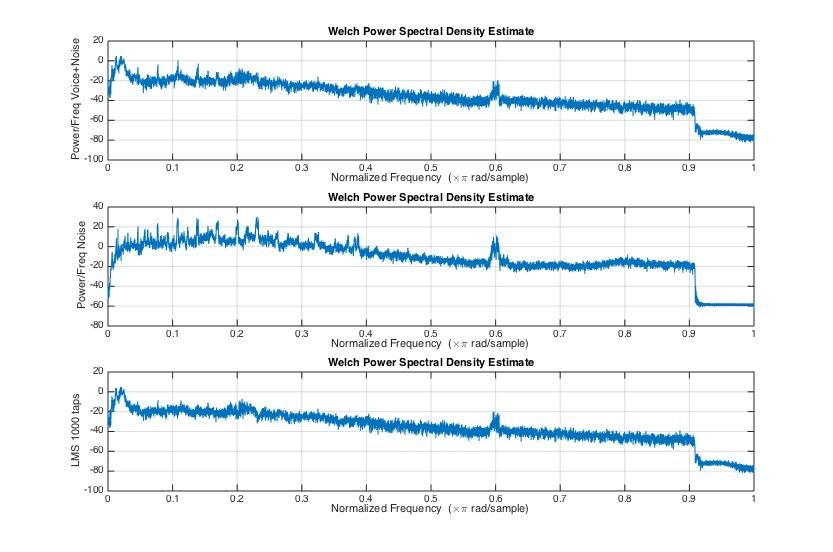
\includegraphics[width=15cm]{images/theory/lms100tapsfreq.jpg}
		\caption{Frequency Domain - LMS result with N=100}
		\label{fig:lmsfreq100}
		\end{figure}
		
		\begin{figure}[h]
		\centering
		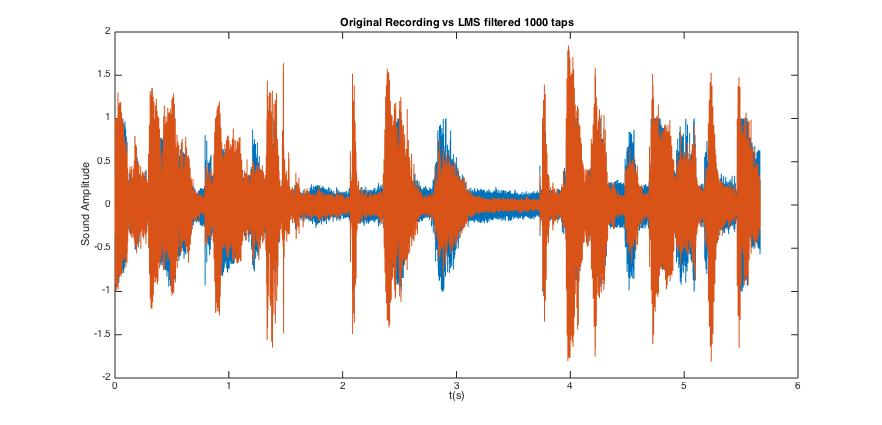
\includegraphics[width=15cm]{images/theory/lms1000tapstime.jpg}
		\caption{Time Domain - LMS result with N=1000}
		\label{fig:lmstime1000}
		\end{figure}
		
		
		\begin{figure}[h]
		\centering
		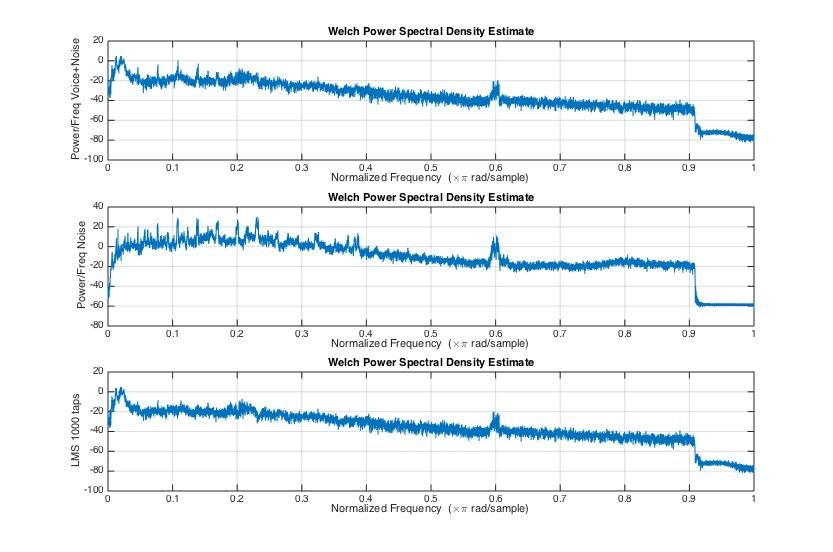
\includegraphics[width=15cm]{images/theory/lms100tapsfreq.jpg}
		\caption{Frequency Domain - LMS result with N=1000}
		\label{fig:lmsfreq1000}
		\end{figure}
		
		
	\subsection{Speech Enhancement Systems: logMMSE}
	\label{sec:enhancement}
	
	\subsubsection{Introduction}
	\label{sec:logmmseintro}
	
The \textit{logMMSE} is a a type of speech enhancement system that, applied after the LMS filter, has been provided the best performance in terms of noise cancellation above all the technique implemented by the theory group with outstanding results of noise cancellation and computational cost.
	
	To be familiar with the term, a speech enhancement system is a transform-based system that uses a single microphone which main goal is speech enhancement. For the outer system, the time domain signal is first framed and windowed.  These frames are generally overlapping. Then a transform, typically \textit{FFT}, is applied to each and every frame. After the processing system, the gain is applied to the transform coefficients and the inverse transform is performed followed by an overlap-and-add method that is to compensate for the windowing and framing \cite{speech}.

	
	The observed signal is given by:

	\begin{subequations}
	\label{eq:speech1}
	\begin{align}
	Y_{k}=\frac{1}{T} \int_0^T y(n) \mathrm{e}^{-j \frac{2\pi}{T} Kt}\,\mathrm{d}t\\
	k=0, 1, 2, \dots	
	\end{align}
	
	\end{subequations}
	
	
	Where \textit{k} denotes Fourier expansion index and \textit{i} denotes time index. The problem here is to estimate the Fourier expansion coefficients of the speech given our noisy speech sequence.

It is naturally assumed by the group that the voice is not always present. Contrary, the noise is considered to be almost always present. Therefore, the main problems to be solved in this type of system are that of estimating the target PSD, i.e. a priori \textit{SNR}, estimating the noise \textit{PSD} estimate and find a suitable statistical assumption for the speech and noise.


In our case, it is assumed that the Fourier Expansion Coefficients can be modelled as statistically independent Gaussian random variables. Both random variables are assumed to be independent in time and in Fourier expansion index. This is motivated by the fact that the Fourier Expansion Coefficients are coefficients that come from weighted random time samples and, through the Central Limit theory, these should approach Gaussian variables. The previous assumptions might not be entirely correct as the windows are overlapping and that there will be dependencies across Fourier expansion coefficients due to windowing, for instance.

The problem in this point is to estimate the Fourier Expansion Coefficients using the \textit{logMMSE}, that stands for logarithmic Minimum Mean Square error function \cite{logmmse}:


	\begin{equation}
	\label{eq:logmmse1}
		\mathrm{E}((log A_{k } - log\hat{A_{k}})^2)
	\end{equation}
	
	This estimator is given by
	
	\begin{subequations}
	\label{eq:logmmse2}
	\begin{align}
		\hat{A_{k}}=exp(\mathrm{E}(ln A_{k}\vert y(t))), t \leq t \leq T\\
		\hat{A_{k}}=exp(\mathrm{E}(ln A_{k}\vert Y_{k}))
		\end{align}
	\end{subequations}
	
	And through the Gaussian model our probability distribution functions are:
	
		\begin{subequations}
	\label{eq:logmmse2}
	\begin{align}
		p(Y_{k} \vert a_{k},\alpha_{k})=\frac{1}{\pi \lambda_{d}(k)} exp(-\frac{1}{\lambda_{d}(k)} \vert Y_{k}-a_{k} e^{j\alpha_{k}}\vert ^2) \\
		p(a_{k}, \alpha{k})=\frac{a_{k}}{\pi \lambda_{k}}exp(-\frac{a_{k}^2}{\lambda_{x}(k)})
		\end{align}
	\end{subequations}
	
	and finally through a whole lot of calculations, we end up with the gain function as follows
	
	
		\begin{equation}
	\label{eq:logmmse3}
		G(\xi_{k},\gamma_{k})=\frac{\xi_{k}}{1+ \xi_{k}} exp(\frac{1}{2} \int_{v_{k}}^\infty \frac{e^{-t}}{t} \mathrm{d}t)
	\end{equation}
	
	The remaining problem is that of estimating the a priori SNR and estimating the noise variance in each frequency bin.
	
For estimating the noise variance, it is used a so-called Voice Activity Detection that tells whenever there is no voice present, and that enables the estimation of only the noise variance, only the noise is present. During moments when there is speech and noise, the noise variance of the past when there is only noise present is used. This is valid if the noise does not change too dramatically. The Voice Activity Detection works by comparing the spectral distance between the noise and the speech.

	
	For estimating the a priori SNR, we use a popular technique which is called decision-directed a priori SNR estimation \cite{speech}.
	
		\begin{equation}
		\hat{\xi_{k}}(n)= \alpha \frac{\hat{A_{k}}^2 (n-1)}{\lambda_{d} (k,n-1)} + (1-\alpha) P(\gamma_{k}(n)-1), 0 \leq \alpha \leq 1
	\end{equation}
	
	
	\[
 P(x) =
  \begin{cases}
   x & \text{if } x \geq 0 \\
   0       & \text{otherwise}
  \end{cases}
\]

Finally, after all the theoretical explanation, the Figure \ref{fig:boxesmmse} shows the block diagram of the running of logMMSE.

		
		\begin{figure}[h]
		\centering
		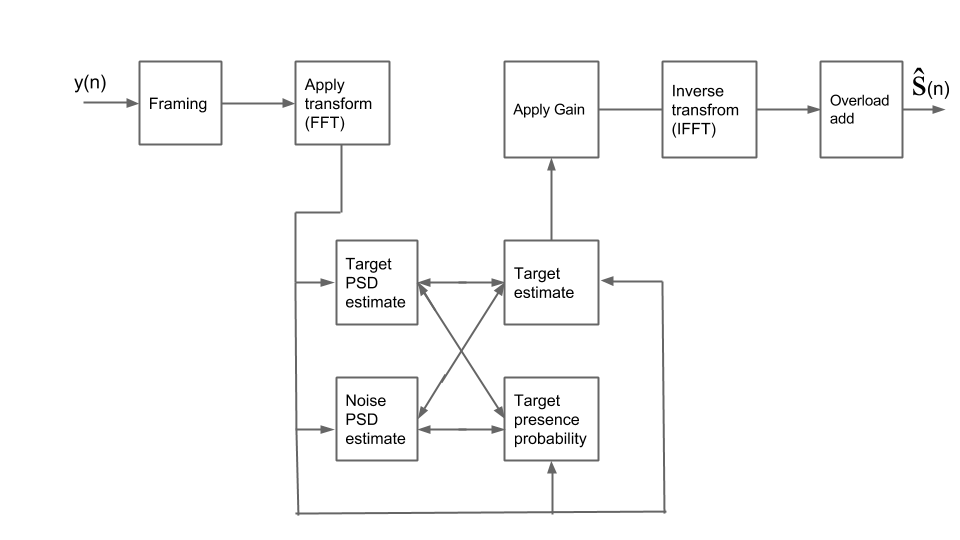
\includegraphics[width=10cm]{images/theory/logmmseboxes.jpg}
		\caption{Box Diagram for logMMSE}
		\label{fig:boxesmmse}
		\end{figure}
		
		This method is one of the simpler ways to estimate the a priori SNR and a very effective one.
	
	\subsubsection{Implementation \& Results}

The implementation in MATLAB of the logMMSE has been done with the help of an already implemented logMMSE function in the website \textit{www.mathworks.com}.

As said in \ref{sec:logmmseintro}, the input of the logMMSE function is the output of the LMS function. In this way, the performance of logMMSE is maximized.

To clarify the utilization of the logMMSE the parameters needed and their values are stated below. In our case, $\alpha=0.99$.

Finally, and using the same kind of analysis than in the previous section, the results will be presented in the time domain and in the frequency domain.

First, Figure \ref{fig:logmmse1} shows the time plots of the different signals: the original, the output of the LMS filter and the output of the logMMSE filter. It can be appreciated that there is a certain unwanted gain in certain parts of the last plot, corresponding to the output of the logMMSE. Even though, this does not affect the quality of the auditive results and, furthermore, the noise is almost 100\% cancelled.

In the Figure \ref{fig:logmmse2} we have the different plots overlapped and it is easier to see how the noise is reduced.


		\begin{figure}[h]
		\centering
		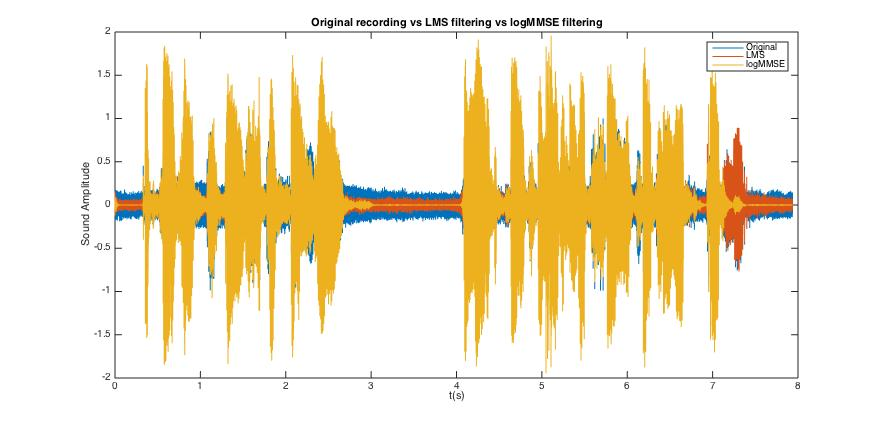
\includegraphics[width=15cm]{images/theory/logmmse2.jpg}
		\caption{Plots of the original signal, the LMS filtered signal and the logMMSE filtered}
		\label{fig:logmmse1}
		\end{figure}
		
		
		\begin{figure}[h]
		\centering
		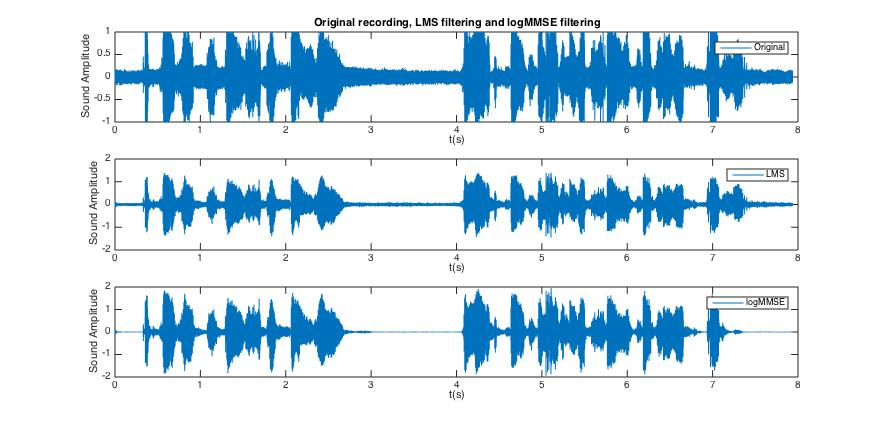
\includegraphics[width=15cm]{images/theory/logmmse3.jpg}
		\caption{Overlapped plots: original, LMS output and logMMSE output}
		\label{fig:logmmse2}
		\end{figure}


Finally, about the computational time, the new system lasts 6 seconds to filter 8 seconds of recording, which makes it efficient and feasible for a transfer to Android to implement a real time application.

	\subsection{Wiener Non-Causal Filtering}
	
	\subsubsection{Introduction}
	
	
	Wiener Filtering is another approach used in Signal Processing with many purposes and noise cancellation is one of them. Inside Wiener Filtering there are many different algorithms to use from which we have chosen Non-Causal infinite dimensional Wiener filtering \cite{asp}.
	
	A general non-causal linear estimator is given by 
	
	
	\begin{equation}
	\label{eq:nonc1}
		\hat{x(n)} = \sum \limits_{k=-\infty}^\infty \theta(n,k)y(n-k)
	\end{equation}
	
	To solve this problem, given the estimator, the group has followed a spectral factorization technique that defines the optimal linear filter as
	
		\begin{equation}
	\label{eq:nonc1}
		H(z)=\frac{\Phi_{xy}(z)}{\Phi_{y}(z)}
	\end{equation}
	
	Therefore, the group's goal is to find $\Phi_{xy}(z)$ and $\Phi_{y}(z)$.
	
	
	\subsubsection{Implementation \& Results}
	
		There are many differences between LMS and Non-Causal Filtering. These are the most important:
		
		\begin{itemize}
		\item Number of phones=2. In this case, to extract the needed information about the noise the third phone that was used to record pure noise is not needed. 
		
		\item The processing is done by frames.
		
		\item A voice unvoice detector is needed.
		\end{itemize}
		
		The developed voice-unvoice detector used is energy-based. As the filtering is done frame by frame, the detector will calculate the variance of the frame and, on behalf of a $\sigma_{ref}$ previously set. A compromise is needed because a high $\sigma_{ref}$ has a good accuracy in the speech detection (less voice presence) but there are some noise frames with part of consonants at the end or the beginning of a noise block. Contrary, a small $\sigma_{ref}$ guarantees a pure noise sample but it adds noise presence in the voiced samples. As a result, we used a high $\sigma_{ref}$, thus what we want to estimate the better is the noise, so it is what we really want to update and filter afterwards.  An example of how the detector works is shown in Figure \ref{fig:detector}.
		
		\begin{figure}[h]
		\centering
		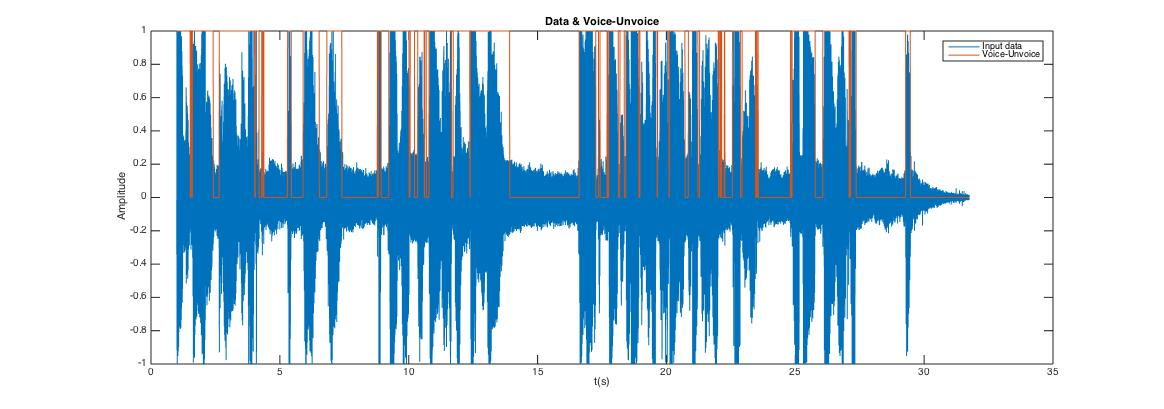
\includegraphics[width=15cm]{images/theory/highsigma.jpg}
		\caption{Voice-Unvoice detector}
		\label{fig:detector}
		\end{figure}
		
		
		Once the frame is decided to be voiced or unvoiced the proper calculation of $\Phi_{xy}(z)$ and $\Phi_{y}(z)$ is next step. To do so, the group has used MATLAB functions used previously in the \textit{Adaptive Signal Processing (EQ2400)} course. These functions require information about the noise and voice frames such as their variances and means. Therefore, to calculate them the MATLAB code follows next steps:
		
		\begin{itemize}
		\item It is assumed that the teleconference starts with a noise frame
			\item Voice-Unvoice detection of the frame
		\begin{itemize}
			\item If the frame is unvoiced: $\mu_{unvoiced}$ and $\sigma_{unvoiced}$ are updated
			\item If the frame is detected as voiced: $\mu_{voiced}$ and $\sigma_{voiced}$ are recalculated and $\mu_{unvoiced}$ and $\sigma_{unvoiced}$ remain equal
			\end{itemize}
			
		\item Filter the frame
			\begin{itemize}
			\item If the frame is unvoiced should be totally removed
			\item If the frame is voiced the noise should be reduced
			\end{itemize}
			\item No overlap between frames
		\end{itemize}
		
		After applying these steps the results have been partly satisfactory. As can be appreciated in the Figure \ref{fig:nonc}, the noise is highly reduced in the unvoiced frames. On the other hand, the drawback comes in shape of unstable regions, as can be seen at first sight between seconds 4 and 5. Figure \ref{fig:noncunstable} shows a zoom in an unstable region, and a possible explanation of it is that the functions used in the non-causal filtering is the inserting of a zero 60 samples-vector at the end of each filtered signal, in each frame in our case.
		
		To try to solve this problem, a solution to filter overlapped frames has been implemented. The main purpose of if was to avoid unstable regions and the zero-sample vectors. Meanwhile the second problem has been successfully solved, a bigger unstable appeared, as shown in Figure \ref{fig:noncunstableoverlap}. A curious results is the perfect shape of a decreasing exponential that it has.
		
		However, the members of the theory group have been working in parallel, while this problem was trying to be solved the performance of \ref{sec:enhancement} gave extraordinary results and the research to solve this problem was stopped.
		
	
		
		\begin{figure}[h]
		\centering
		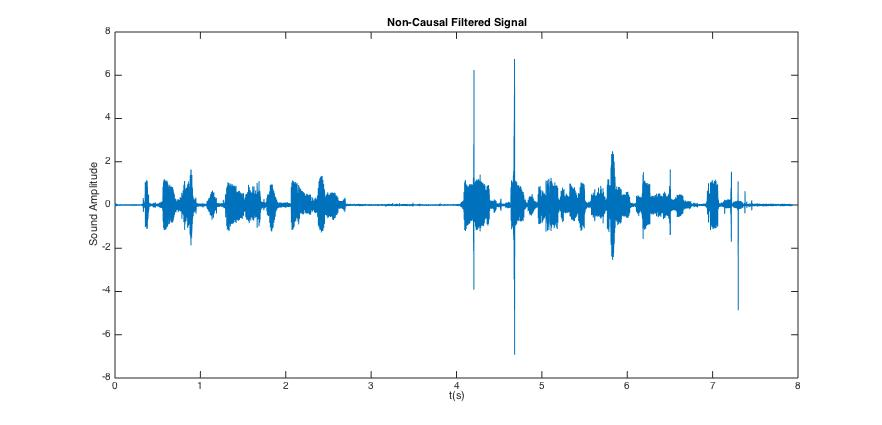
\includegraphics[width=15cm]{images/theory/nonc.jpg}
		\caption{Unstable region in non-causal filtering}
		\label{fig:nonc}
		\end{figure}		
		
		\begin{figure}[h]
		\centering
		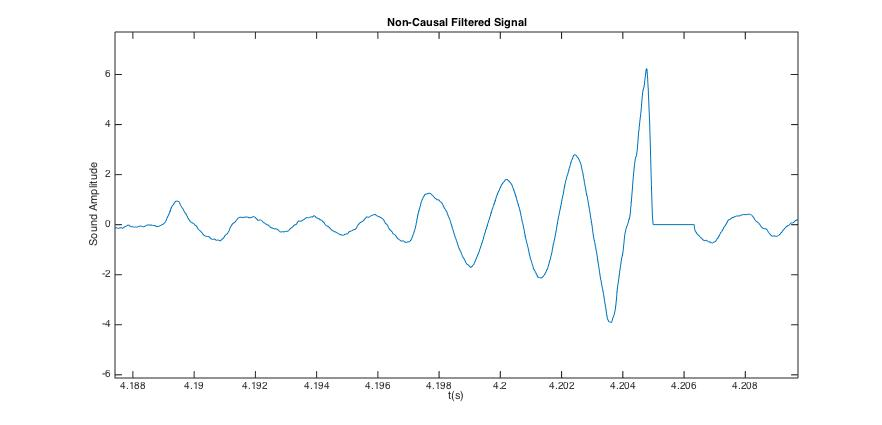
\includegraphics[width=15cm]{images/theory/noncunstable.jpg}
		\caption{Unstable region in non-causal filtering}
		\label{fig:noncunstable}
		\end{figure}
		
		\begin{figure}[h]
		\centering
		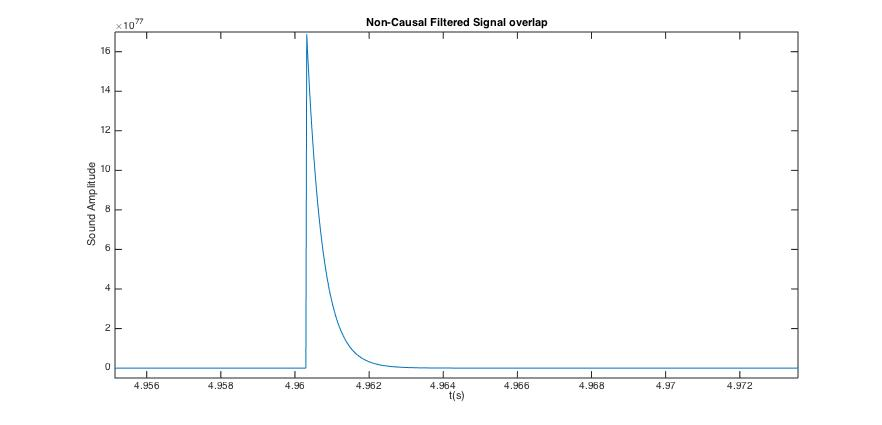
\includegraphics[width=15cm]{images/theory/noncunstableoverlap.jpg}
		\caption{Unstable region in non-causal filtering}
		\label{fig:noncunstableoverlap}
		\end{figure}		
	


\section{Unsuccessful Approaches}

In this section some of the unsuccessful approaches of the theory group are presented. The reasons of the unreached success come from different natures, as will be explained above in each algorithm or technique.

	\subsection{Kalman Filtering}
	Kalman Filtering is an Adaptive Filtering technique highly used in tracking and predicting, for instance. Therefore it was considered as a suitable option to face the noise cancellation problem of this project. But, unfortunately this technique showed two main drawbacks:
	
	\begin{itemize}
	\item Computational cost too high. Therefore it is not possible to transfer to the Android coding.
	\item Difficulties to find a right State-Space Model showed in Equation \ref{eq:kalman}, i.e. problems to find \textit{F, G, H, v(n) and w(n)}
	\end{itemize}
	
	
	\begin{subequations}
	\label{eq:kalman}
	\begin{align}
	x(n+1)=Fx(n)+Gw(n)\\
	y(n)=Hx(n)+v(n)	
	\end{align}
	
	\end{subequations}
	
	For the reasons above, this way was dropped in the first weeks of the project.
	
	\subsection{RLS}
	
	The Recursive Least Squeares (RLS) Algorithm \cite{asp} is supposed to have a better convergence and result than the LMS Algorithm. The problem that RLS tries to solve is the FIR Wiener one, where the aim is to estimate the process $x(n)$ using a fixed number of observations from another process ${y(n)}$ using a liner estimator
	
	\begin{equation}
	\hat{x}(n)=\sum \limits_{k=-0}^{N-1} \theta(k)y(n-k)=Y^T (n)\theta
	\end{equation}
	
	where $Y(n)= [y(n),y(n-1),\dots,y(N-N+1)]^T$ are the samples that have to be filtered and the crierion is $MSE(\theta)=E{(x(n)-\hat{x(n)})^2}$.
	
	Nevertheless, the option was tested during the first days of the project and dropped after checking the Computational Cost: O($N^2$) vs the  O($N$) of the LMS.
	
	
	\subsection{Frequency Domain LMS-Algorithm}
	
	One of the main reasons why the \textit{Frequency Domain LMS-Algorithm} was considered was due to the fact that the time domain algorithm required a lot of taps, in the order of a 1000 taps, which made the amount of multiplications per sample very high. 
	
What the frequency domain LMS does is that it works in the frequency domain and takes blocks of data and process, instead of processing sample by sample, like in the time domain LMS, which means that the amount of multiplications per sample drastically decreases, by up to 16 times. The frequency domain LMS is often used for noise cancellation, hence there are a lot of research on this topic, but not for noise cancellation purposes.

The issue with the frequency domain LMS is the fact that it does not converge as fast as time domain algorithm, which means that a lot of noise will not be removed. Another problem is that the blocks must be windowed and overlapped and after processing, one must use the overlap and add method and all of this increases the amount of computations per sample. To have a better understanding about the \textit{Frequency Domain LMS-Algorithm}, the Figure \ref{fig:freqlms} shows the block diagram of this technique.


		\begin{figure}[h]
		\centering
		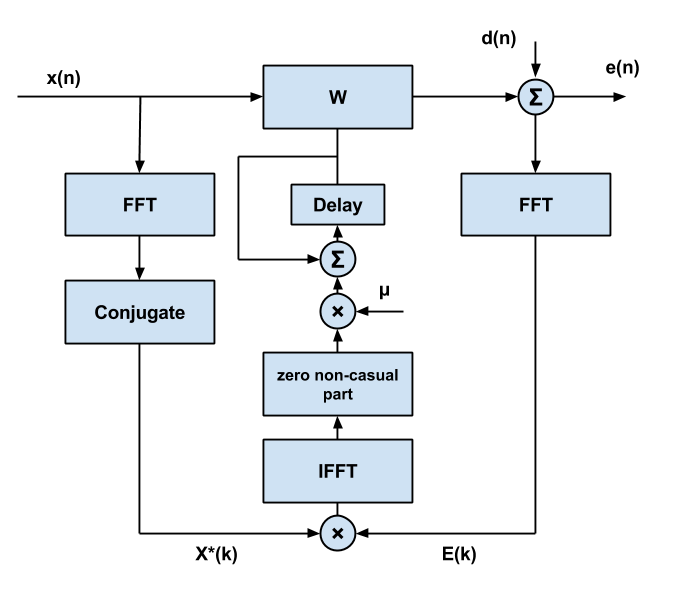
\includegraphics[width=10cm]{images/theory/freqlms.jpg}
		\caption{Frequency Domain LMS-Algorithm Block Diagram}
		\label{fig:freqlms}
		\end{figure}


\chapter{Android}

The Android part has been the most challenging in the whole project: implement a real time application with signal treatment implies code optimisation skills. Even though Android environment coding was a new experience for all the members of the group, the results have been outstanding.

The coding environment of Android is Eclipse and the language used is JAVA, object oriented and assumed to be known by the reader. Moreover, the used \textit{Android} platform is \textit{Android 5.1}. 

As a clarification, the framework used in the project was the one provided by the supervisor, Per Zetterberg.

In this chapter the followed steps and reached results during the performance of the project are presented. 

\section{Learning Android}

For the \textit{Android Group}, the project began with a set of tasks that needed to be finished before the \textit{Midterm Evaluation}. It goes without saying that the group did it in less time than expected and could start working on the transfer from MATLAB to Android coding two weeks earlier than expected.

\section{Coding for Noise Cancellation}
\label{sec:coding}

Once the group was familiarized with the environment, the procedure of processing the information needed to be set. As the communication path for the teleconference is the Internet, the information is going to be sent with TCP frames, therefore the signal processing is going to be frames/blocks oriented, i.e. buffering is needed for such an application. The solution that has been kept for the buffering is: to use dynamic lists of buffers.

In terms of time, the buffer is a constant parameter and it lasts around \textit{92 ms}. Contrary, the buffer length, in terms of number of samples, is frequency $f_{s}$ dependent and proportional. Typical buffer lengths are $1024$ and $2048$ samples which correspond to \textit{$f_{s}$=11025 Hz} and \textit{$f_{s}$=22050 Hz} respectively.


	\subsection{State Diagram}
	
	To have a full understanding about how does the coding work, it is necessary to define a state machine diagram (see Figure \ref{fig:states}). The list of states and their explanation are above:
	
	\begin{itemize}
	\item \textbf{Waiting}: starting state. This state is used to wait for both signal and noise phone to be online and to send buffers. Then, the buffers are filled until T1 happens.
	
	\item \textbf{Correlation}: state where the cross-correlation between the signal and noise buffers is calculated. The maximum of the cross-correlation gives the total delay between the two samples’ flows. Then, by a simple algorithm, this total delay is divided into two variables. These two variables are important thus the coding works with dynamic lists of buffers. The two variables are:
	
		\begin{itemize}
		\item \textit{Number of buffers between the two corresponding buffers}: this is the number of buffers needed to throw, either for the signal or the noise, to synchronize the buffers' lists.
		\item  \textit{Delay inside the synchronized buffers}: this is the number of samples we need to throw, either for the signal or the noise, to synchronize the samples.
		\end{itemize}
		
	\item \textbf{Empty}: useless buffers (used for the cross-correlation) are removed. This state also helps fixing the length of the dynamic lists.
	
	\item \textbf{Play}: the most complex state. It can be divided as follows:
	
		\begin{itemize}
		\item \textit{Initialization phase}: variables that will be used are initialized, particularly the noise, signal and \textit{to\_be\_played} arrays. The \textit{to\_be\_played} array is basically the same as the signal array,  but of a smaller length since more samples are needed on the signal array to apply the \textit{NLMS Algorithm}, otherwise some samples could be missed.
		
		\item \textit{Noise cancellation phase}: the algorithm goes through this phase if we ask it to do it; otherwise it skips to the next phase. This phase applies the NLMS algorithm between the signal and the noise arrays. Then the result is subtracted to the \textit{to\_be\_played} array.
		
		\item \textit{Voice detection phase}: this algorithm uses the \textit{to\_be\_played} array (after NLMS or not) to detect if there is voice or not. If there is no voice, some parts of the array are set to zero.
		\item \textit{Playing phase}: the processed array \textit{to\_be\_played} is played and some checking variables are updated
		\end{itemize}
		
		
	\end{itemize}
		
		Once the states are explained, the transitions are the last concepts to have a full understanding of this section:
		
		\begin{itemize}
		\item T1: happens when enough buffers are received from the signal and the noise phones to calculate the cross correlation between the buffers.
		\item T2: happens when the cross-correlation has been calculated and the delay computed.
		\item T3: happens when the useless buffers are removed (the one we used to calculate the cross-correlation)
		\item T4: happens when someone tap the button \textit{re-init} on the phone’s screen.
		\end{itemize}


		\begin{figure}[h]
		\centering
		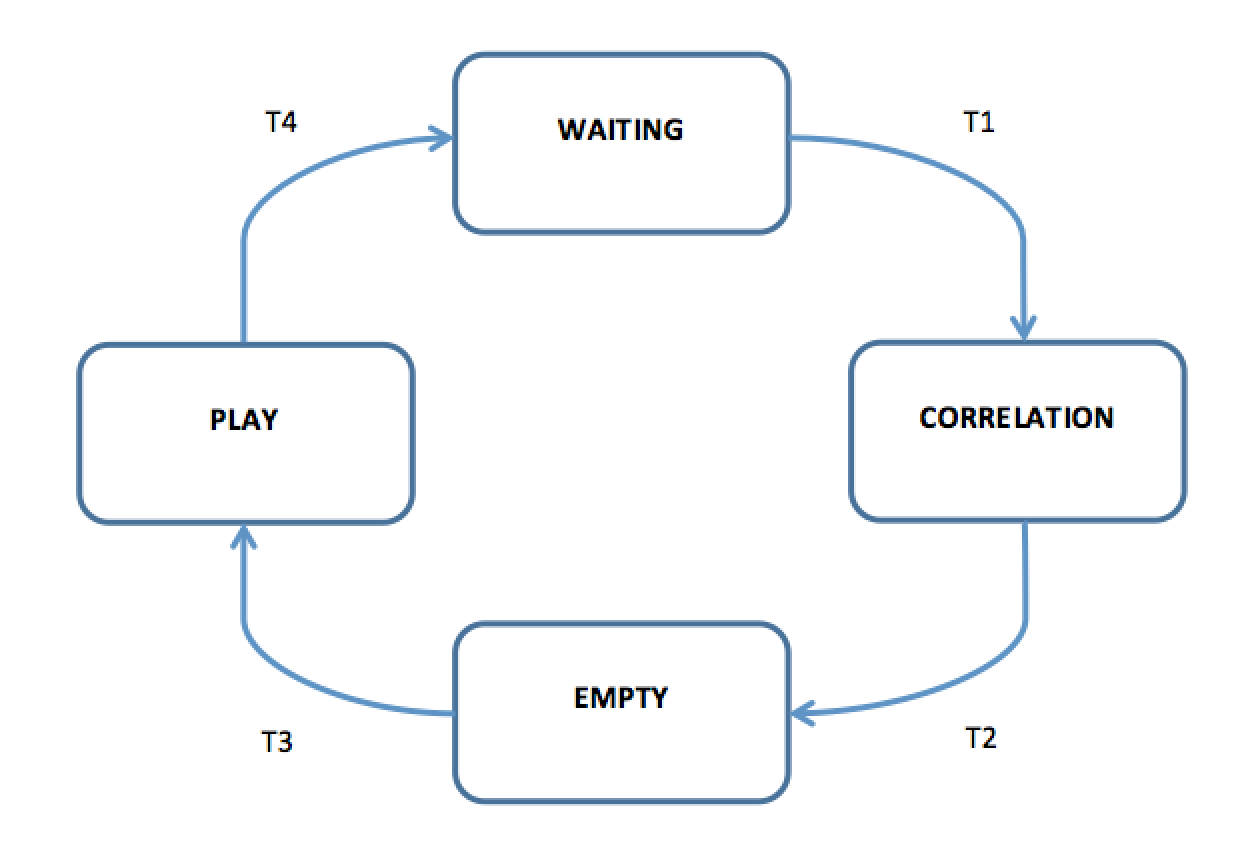
\includegraphics[width=10cm]{images/android/states}
		\caption{State Diagram in the Android Coding}
		\label{fig:states}
		\end{figure}	
		
		
		\subsection{NLMS}
		
		The proposed LMS solution by the \textit{Theory Group} ended up with several problems when it was translated to JAVA. One of the problemas was the presence of saturation. Therefore, the \textit{Android Group} needed to do some changes in the code.
		
		As a possible explanation, few problems that may appear on the LMS are related to stability due to the signal's power. Hence the step-size may have to be chosen unnecessarily small. However, the LMS can be made insensitive to the signal power by using a normalized step-size \cite{asp}:
		
		
		
	\begin{equation}
	\label{eq:nlms}
		\mu (n)=\frac{\bar{\mu}}{c+\lVert Y(n)\rVert^2}
	\end{equation}
	
	The NLMS version in Android has been challenging because the buffers used on the framework last approximately \textit{92 ms}, as commented in \ref{sec:coding} and the processing part has to last less than this time. Because the NLMS version was imported from MATLAB, it has been first translated to JAVA and later on the code has been improved to reduce the execution time. These have been two implemented solutions to do so:
	
	\begin{itemize}
	\item \textbf{Intelligent 'for-loops`}: The for-loop executes a test on the index variable for every iteration. This test consists of calculating the subtraction between the index variable and the tested value, and then compare it to $0$. To really reduce the execution time, the compared value has to be zero and thus no subtraction will be calculated, which helps if there are a lot of iterations. It is done as follows:
	
		\begin{itemize}
			\item Replacing
			
\begin{lstlisting}
for(int i=0;i<bufferLength;i++){
//Calculation
}
\end{lstlisting}
			
			\item With
			
\begin{lstlisting}
int i;
for(i=bufferLength;i-->0;){
//Calculation
}

\end{lstlisting}
	
		\end{itemize}
	
	\item \textbf{Moving every “static” calculation out the loops:}  operations inside loops take time. Therefore, all the constant with to the loop index are taken out of the loop and define them as local variables to avoid useless calculations. It costs less to point at a local variable than to calculate.
	
	\begin{itemize}
	\item Replacing:
	
\begin{lstlisting}
toFilter=new int[bufferLength];
int i;
int x=10;
int y=2;
for(i=bufferLength;i-->0;){
	toFilter[i]=x*y;
}
	
\end{lstlisting}
		
		\item With:
		
\begin{lstlisting}
toFilter=new int[bufferLength];
int i;
int x=10;
int y=2;
int z=x*y;
for(i=bufferLength;i-->0;){
	toFilter[i]=z;
}

\end{lstlisting}

	\end{itemize}
	
	\item \textbf{Do not instantiate inside the loops}: Everything is said in the title. If the coded is translated directly from MATLAB, the code might end up with variables that are instantiated inside loops. This is a situation to avoid. To instantiate variables takes some precious time for real time application.
	
	\begin{itemize}
	\item Replace:
\begin{lstlisting}
for(i=bufferLength;i-->0;){
	int x=0;
	//Processing that uses x
}

\end{lstlisting}

	\item With:
	
\begin{lstlisting}
int i;
int x;
for(i=bufferLength;i-->0;){
	x=0;
	//Processing that uses x
}

\end{lstlisting}
		\end{itemize}

	
		\end{itemize}
	
	It is important to say that the \textit{Android Group} has achieved the results using only an LMS of order 10, much inferior to the orders 100 and 1000 initially proposed by the \textit{Theory Group}.

	
	\section{The Application}
	
	This section aims to be an explanation and graphic demonstration of the application interface developed by the \textit{Android Group}. The main purpose of the application is to make the noise cancellation work correctly.
	
	Neither the layout nor the functionality are meant to a commercial use thus there are options like changing the value of the step-stize of the \textit{LMS Algorithm}. Consequently, the app is designed to be used in an engineering lab environment.
	
	
	\subsubsection{Screens of the application}
	
	The application's interface with the user consists in 3 main different screens. The Figure \ref{fig:starting} shows the first screen (\textit{Starting Screen}) that appears when the app is launched. At this point, to continue it is necessary to tap the screen to jump to the \textit{Selection Screen} shown in Figure \ref{fig:selection}.
	
	The \textit{Selection Screen} show the different roles that the mobile phone can have:
	
	\begin{itemize}
	\item Sender: it is the phone used by the user in the noisy environment.
	\item Noise: it is the phone that collects the noise information necessary to apply the \textit{LMS Algorithm}
	\item Receiver: it is the phone of the receiver. This phone is the one in charge of the noise cancellation
	\end{itemize}
	
	
	Finally, the last important screen is the \textit{Receiver Screen}. This is the screen displayed in the receiver phone from where some of the parameters of the noise cancellation algorithms will be managed. There are two main parts in this screen, one for parameters or mode selection and the other one of pure information.
	
	On the one hand, the \textit{Receiver Screen} has different option buttons:
	
	\begin{itemize}
	\item Blue button: decides whether apply the noise cancellation or not
	\item Orange button: decide whether we apply the voice detection or not
	\item Green and red buttons: add the written values to $\mu$ (step-size)
	\item Yellow button: re-initialize the application (we go back to the WAITING state)
	\end{itemize}
	
	On the second hand, there is a second part in the \textit{Receiver Screen} that display all the necessary values to have a full understanding about what is the application doing:	
	
	\begin{itemize}
	\item \textit{mu} (step-size): this is the value of the $\mu$ coefficient
	\item \textit{mu'} (normalize step-size): this is the modified value of $\mu$ used for the  \textit{NLMS Algorithm}
	\item \textit{Diff}: number of buffers between two synchronized buffers (one from sender and one from noise)
	\item \textit{Delay}: the delay inside two synchronized buffers in number of samples
	\item \textit{totalDelay}: it’s the total delay observed in number of samples
	\item \textit{noiseCancellation}: Boolean that tells if we apply the noise cancellation or not
	\item \textit{VD}: Boolean that tells if we apply the voice detection or not
	\item \textit{speechFlag}: Boolean that tells if we detected speech or not
	\item \textit{timeVD}: execution time of the voice detection algorithm
	\item \textit{timeLMS}: execution time of the NLMS algorithm
	\item\textit{lengthSenderBuffer}: length of the ArrayList containing the recorded buffers from the sender
	\item \textit{lengthNoiseBuffer}: length of the ArrayList containing the recorded buffers from the noise
	\item \textit{Number of taps}: obviously this is the order of the NLMS filter.
	
	\end{itemize}

	
	
		\begin{figure}[h]
		\centering
		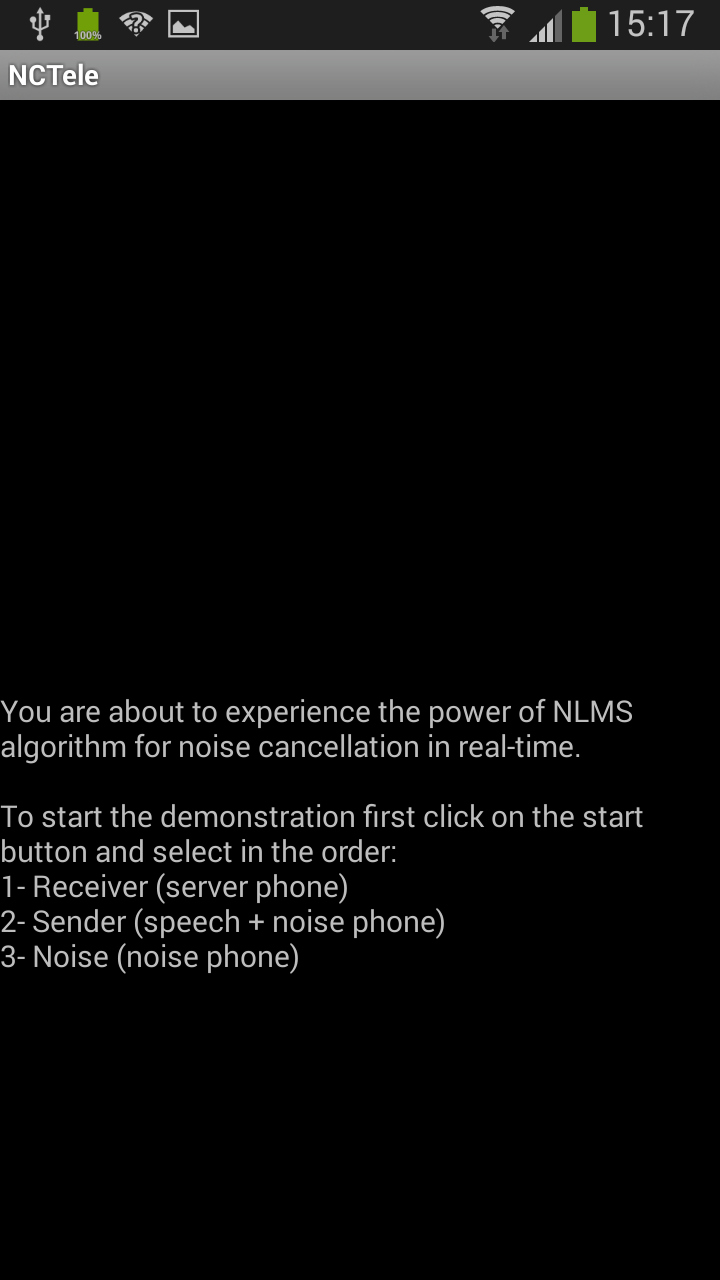
\includegraphics[width=6cm]{images/android/startingscreen.jpg}
		\caption{App's starting screen}
		\label{fig:starting}
		\end{figure}
		
		
		\begin{figure}[h]
		\centering
		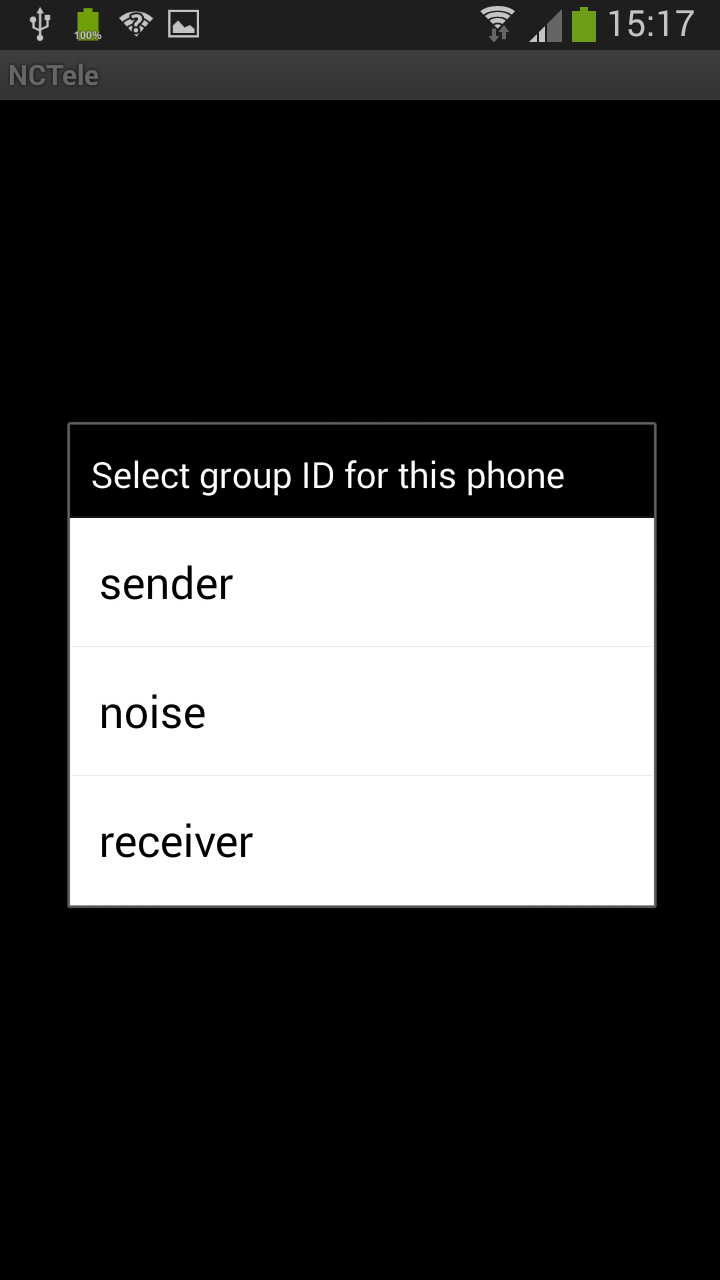
\includegraphics[width=6cm]{images/android/selectionscreen.jpg}
		\caption{Selection of role in the teleconference}
		\label{fig:selection}
		\end{figure}
			
		
		
		\begin{figure}[h]
		\centering
		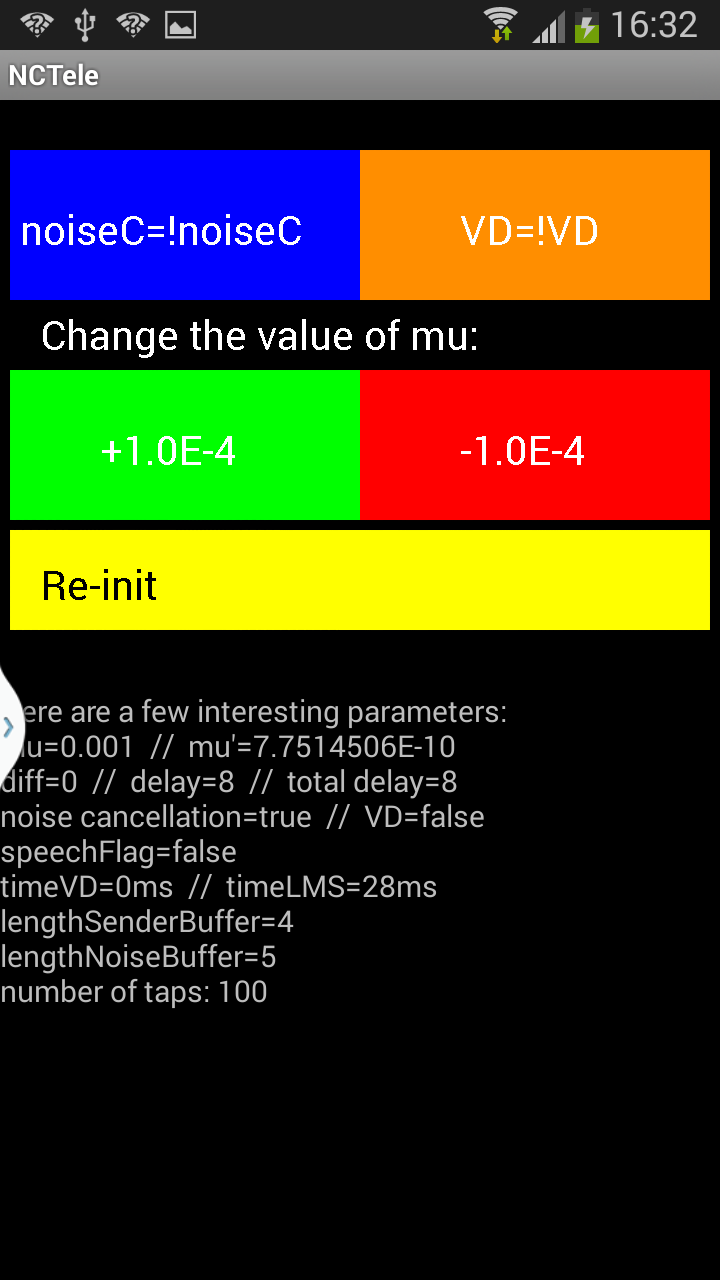
\includegraphics[width=6cm]{images/android/receiverscreen.jpg}
		\caption{Receiver screen: noise cancellation parameters selection}
		\label{fig:receiver}
		\end{figure}
	

\chapter{Conclusions}

The evaluation of the project as whole is absolutely positive. Nevertheless, the group does not consider it a complete success due to several problems or limitations that it has.


\section{Theory Conclusions}
From a theoretical point of view, the noise cancellation has been achieved in MATLAB simulation with non appreciable distortion or voice modification. Moreover, the techniques used to do so have been successful and computationally efficient, which was a requirement before transferring the code to Android.

As a conclusion, the group has seen that combination of different techniques gives better results.

\section{Android Group}
The challenge of the Android has been partially achieved. In terms of communications, the two phones connect to each other with an acceptable delay. On the other hand, the system is limited to a static position, i.e. both phones that are involved with the noise need to remain in the same position for synchronisation purposes.

The synchronisation has been one of the bigger problems. As a main requirement for the NLMS usage, it is necessary a maximum correlation between the noise samples that arrive to the receiver from the sender and the ones from the noise recorder. Otherwise, the NLMS performance is limited (\ref{lms}). Therefore, the required synchronisation will be done by correlation.

The biggest problem concerning synchronisation is the distance between the phone of the \textit{Speaker 1} and the phone of the \textit{Noise}. This distance will affect directly to the delay between the signals when they will arrive to the phone of the \textit{Speaker 2}. This delay is due to the propagation of the acoustic waves in the air. For instance, considering that the sound propagation in the air is $v_{air}=340$ \textit{m/s}, with a \textit{5 m} distance between these two phones, the delay is $\Delta_{t}=14.7$ \textit{ms}. This delay has a real impact on the required size of the filter. Taking next values into account:

\begin{itemize}
\item $f_{s}=11$ \textit{KHz} (Minim possible value)
\item $t_{buffer}=92$ \textit{ms} (Buffer duration)
\end{itemize}

and doing the proper calculations ($order_{minim}=\frac{14.7}{92} \cdot 1024=163$) samples. Finally, with this set up, 163 is the minimum degree of the NLMS Filter.

On the other hand, with a 100 degree NLMS filter the voice received by the \textit{Speaker 2} suffers noise distortion, possibly because of Inter Symbol Interference.

With this results, the group has faced a trade-off between the noise cancellation and the voice distortion. Thus, the final set up is as follows:

\begin{itemize}
\item Distance between phones: 0.5 m (maximum)
\item Order of the NLMS filter: from 10 to 50
\end{itemize}

As a result, the noise cancellation is considered a success and the received voice suffers a smaller distortion.

Moreover, there is a special set up that has given extraordinary results. This set up consists of two phones besides each other, being one as the \textit{Noise phone} and the other one as the \textit{Speaker 1 phone}. As a result, the \textit{Speaker 2} can experience a full noise cancellation. The Figure \ref{fig:setup} shows the mentioned set up.

		\begin{figure}[h]
		\centering
		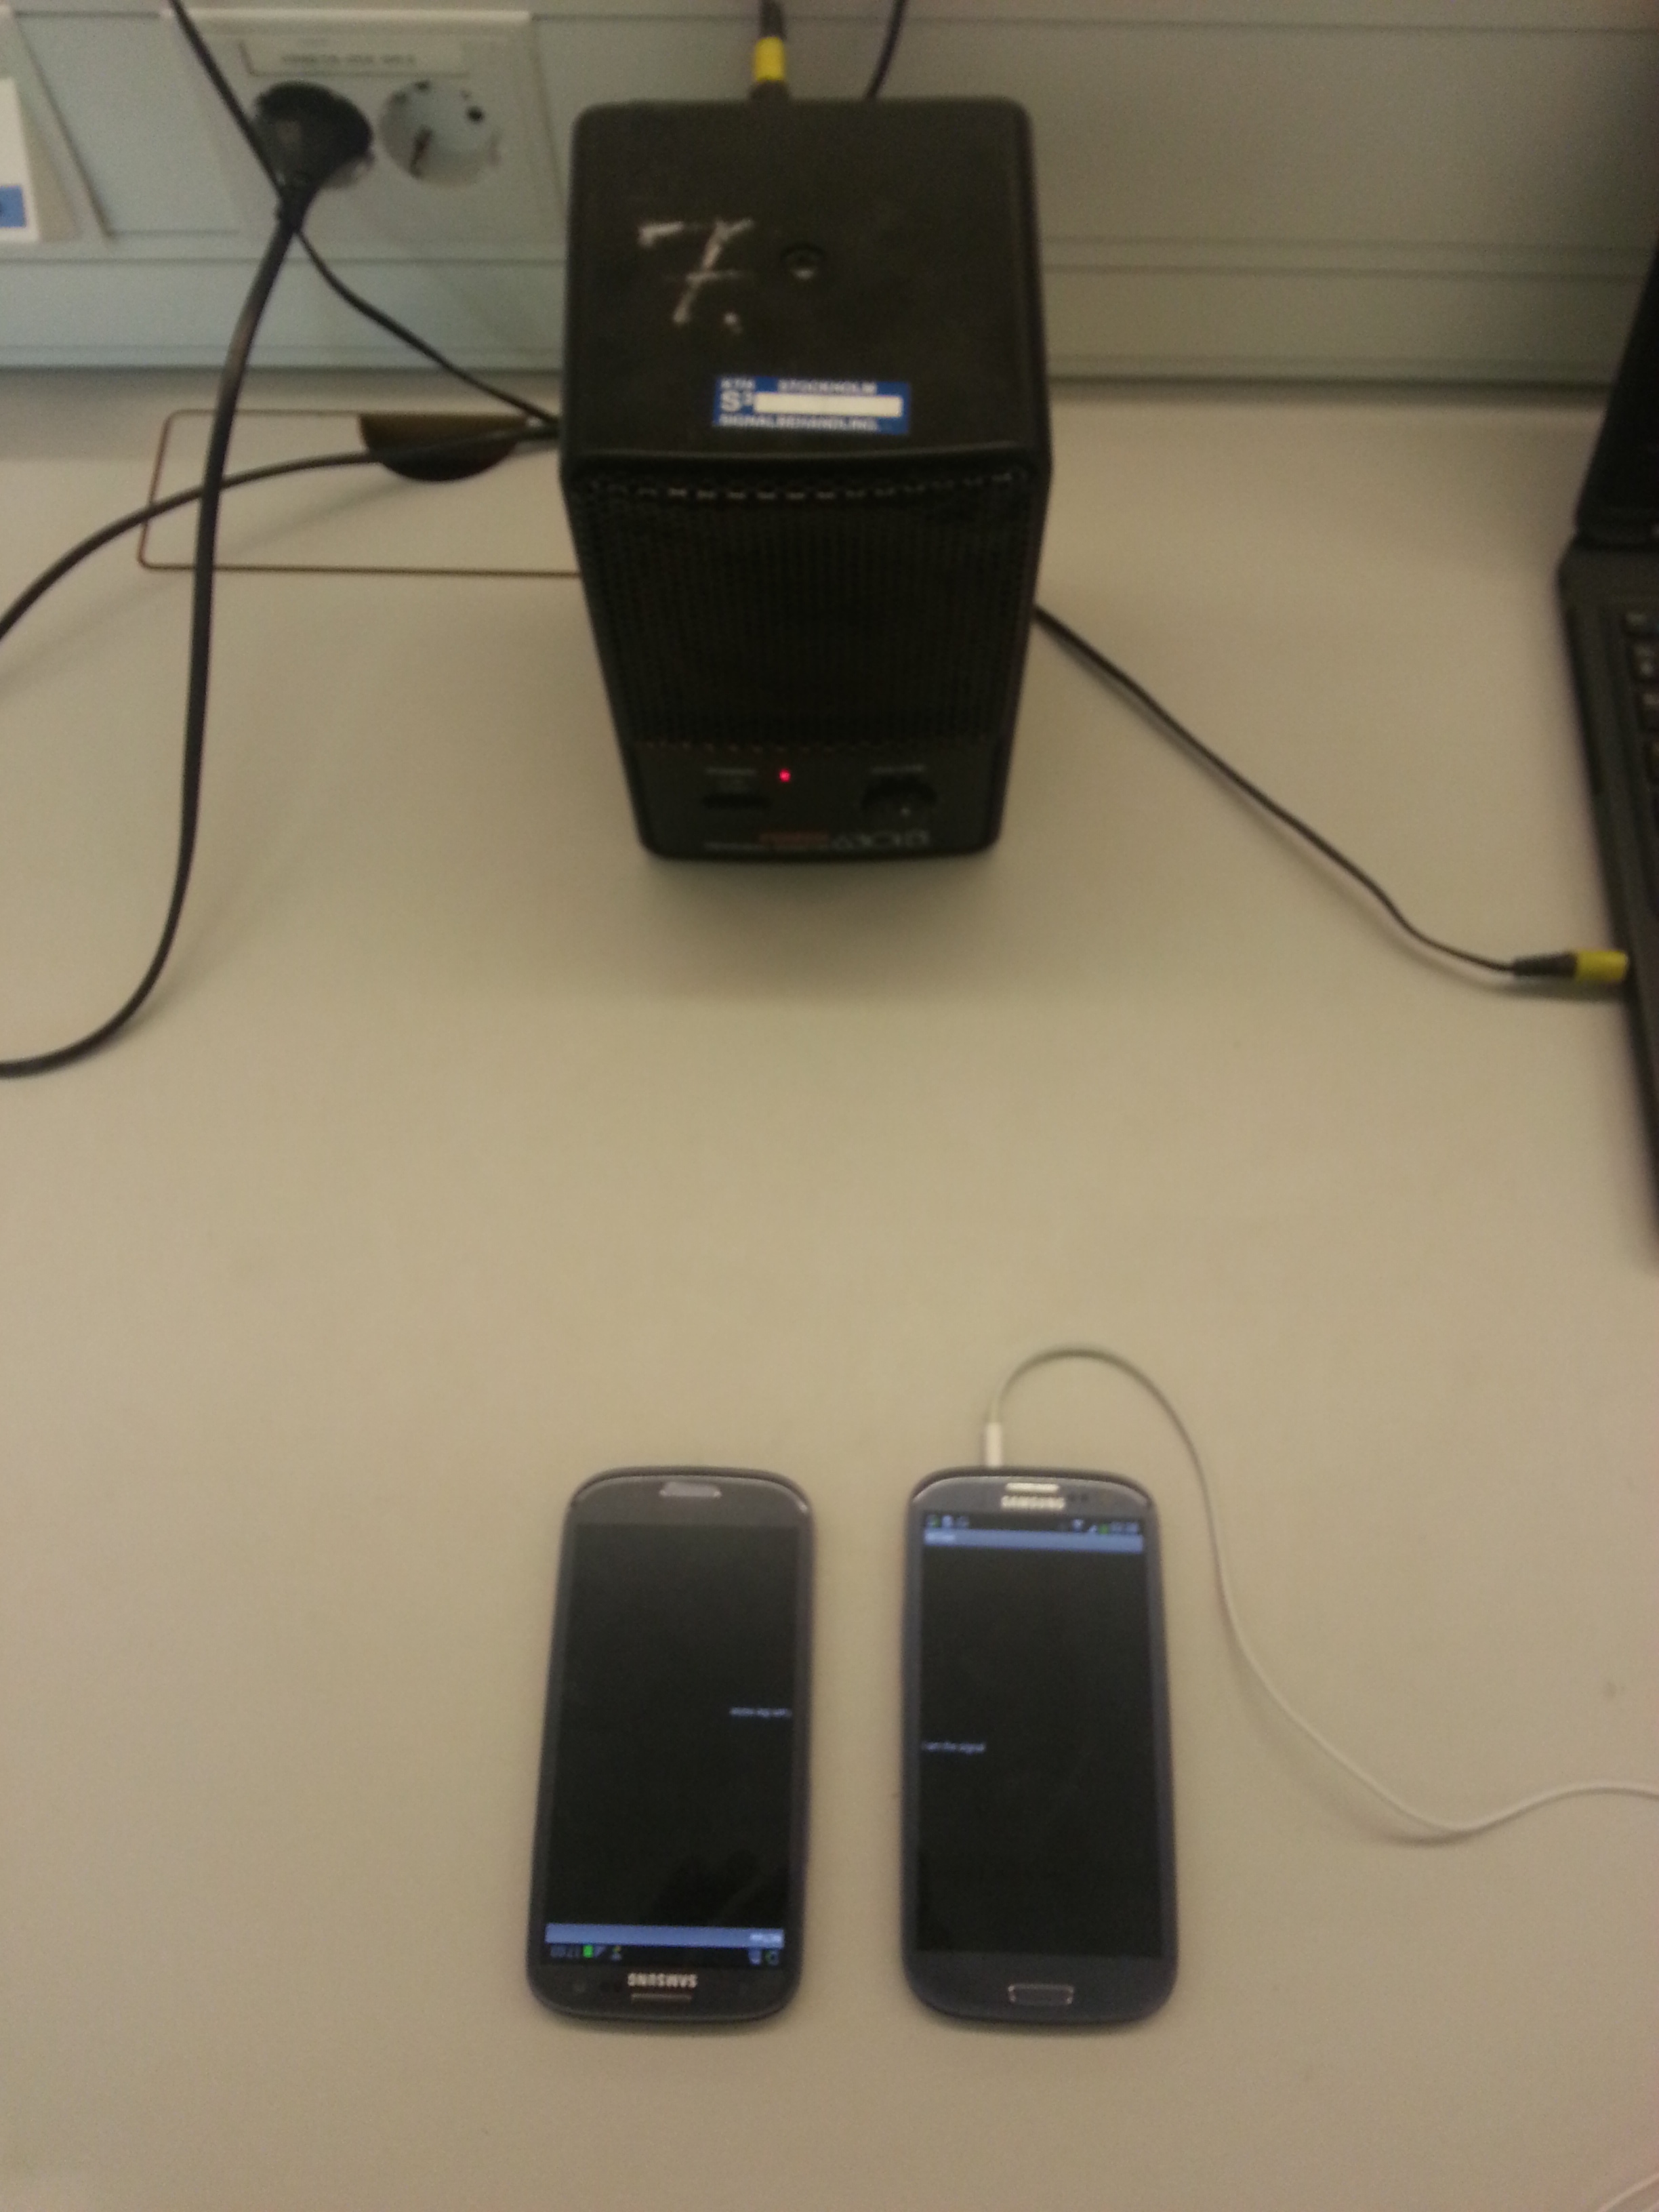
\includegraphics[width=6cm]{images/android/setup.jpg}
		\caption{Set up for complete noise cancellation}
		\label{fig:setup}
		\end{figure}


\section{Open issues to solve}

Taking into account all the problems found out during the performance of the project and the limitations of the final application, the \textit{Group} will list the open issues to solve as proposals to continue the project:

\begin{itemize}
\item Reach a non-static set up of the phones
\item Reach phonic isolation between the noise and the senders phone
\item Reach maximum correlation between the added noise to the teleconference with the pure noise signal 
\end{itemize}



\chapter{Appendices}
\label{sec:appendix}


\bibliographystyle{plain}
\bibliography{ref}

%\include{Chapter1}			% Incluye "Chapter1.tex"


%%%%%%%% Fin del documento %%%%%%%% 
\end{document}
